\documentclass[conference]{IEEEtran}
\IEEEoverridecommandlockouts
\usepackage{cite}
\usepackage{amsmath,amssymb,amsfonts}
\usepackage{graphicx}
\usepackage{booktabs}
\usepackage{multirow}
\usepackage{xcolor}
\usepackage{tikz}
\usetikzlibrary{positioning,arrows.meta,fit,calc,shapes.geometric}
\usepackage[hidelinks]{hyperref}
\usepackage{url}
\graphicspath{{figures/}{../outputs/}}

\newcommand{\repo}{\url{https://github.com/Quttoshi/moe-image-restoration}}
\newcommand{\video}{\url{https://youtu.be/VIDEO_ID}}
\newcommand{\todo}[1]{\textcolor{red}{[TODO: #1]}}

\tikzset{
  blk/.style={draw, rounded corners=2pt, minimum height=6mm, minimum width=9mm, align=center, font=\scriptsize},
  enc/.style={blk, fill=blue!10},
  dec/.style={blk, fill=green!10},
  lat/.style={blk, fill=orange!20},
  arr/.style={-{Latex[length=1.5mm]}, thick},
}

\begin{document}

\title{From Universal Autoencoders to Soft Mixtures of Experts and Style-Conditioned GANs:\\
Image Restoration and Face-to-Sketch Generation\\
\large Generative AI -- Assignment 1}

\author{\IEEEauthorblockN{Shehbaz (21i2525), Section A}
\IEEEauthorblockA{Code: \repo}}

\maketitle

\begin{abstract}
We build, tune and deploy four related generative systems. Three of them restore $128\times128$
Oxford-IIIT Pet images corrupted at runtime by salt-and-pepper noise, Gaussian blur or rectangular
occlusion: (i) a single universal denoising autoencoder with a genuine compressed bottleneck; (ii) a
hard-routing system in which a four-way corruption classifier dispatches each image to one of three
specialist autoencoders or to an identity bypass; and (iii) a differentiable soft mixture-of-experts
(MoE), initialised from (ii) and fine-tuned jointly with reconstruction, structural-similarity,
classification and routing-balance losses. The fourth system is a style-conditioned pix2pix
generator that turns FS2K facial photographs into sketches in one of three artistic styles, with a
learned style embedding in both the U-Net generator and the PatchGAN discriminator. Every model is
tuned with Optuna, tracked in MLflow, exported to ONNX with verified numerical parity,
and served by a FastAPI/ONNX-Runtime backend behind a React and Tailwind interface; the application
starts with a single Docker Compose command. On 36,690 deterministic test cases the universal
autoencoder raises mean PSNR on corrupted inputs from 19.3\,dB to 24.6\,dB (SSIM 0.63$\to$0.79), and the
corruption classifier reaches 99.8\% accuracy (macro-F1 0.997). Hard routing and the soft MoE match
the universal model on corrupted inputs (24.3 and 24.2\,dB) while leaving clean images almost
untouched (SSIM 0.997--0.998 vs.\ 0.847). The learned gate converges to near-hard routing and hedges
only on low-severity and mixed corruptions. Because of the deadline, all Optuna budgets are small, and
we report them as such.
\end{abstract}

\begin{IEEEkeywords}
denoising autoencoder, mixture of experts, image restoration, conditional GAN, pix2pix, Optuna, ONNX
\end{IEEEkeywords}

%=====================================================================
\section{Introduction}
%=====================================================================
Real-world images are often degraded in ways the downstream system cannot know in advance. Two
broad strategies exist. A single \emph{universal} model can learn a shared representation that undoes
every degradation~\cite{li2022airnet,potlapalli2023promptir}. Alternatively, the problem can be
\emph{decomposed}: identify the degradation, then apply a specialist. Hard decomposition is
interpretable but fragile when the identification is wrong. Soft decomposition through a mixture of
experts~\cite{jacobs1991moe,shazeer2017moe} keeps the specialists and replaces the discrete decision
with a learned, differentiable weighting.

This report compares the three strategies under one controlled protocol (Sec.~\ref{sec:data}). It
then addresses a different generative problem: paired, style-conditioned image-to-image translation
from faces to sketches with a conditional GAN~\cite{mirza2014cgan,isola2017pix2pix}. For each task we
describe the alternatives considered, the Optuna search, quantitative and visual results, and the
failure cases. Section~\ref{sec:app} describes the deployed software product.

%=====================================================================
\section{Related Work}
%=====================================================================
\textbf{Denoising autoencoders.} Vincent et al.~\cite{vincent2008dae} showed that reconstructing clean
inputs from corrupted ones yields robust representations. Convolutional encoder--decoders with
symmetric skip connections (RED-Net~\cite{mao2016rednet}, U-Net~\cite{ronneberger2015unet}) and
residual CNNs (DnCNN~\cite{zhang2017dncnn}) dominate restoration. Their skips, however, carry
corrupted detail straight to the output and remove the information bottleneck. The brief forbids
unrestricted skips, so we treat skips as an ablation (Sec.~\ref{sec:t1}). Zhao et al.~\cite{zhao2017loss}
showed that L2 loss correlates poorly with perceived quality and that an L1+MS-SSIM mixture works
better, which motivates our $\alpha$-weighted L1+SSIM objective~\cite{wang2004ssim}.

\textbf{All-in-one restoration.} AirNet~\cite{li2022airnet} learns a degradation representation by
contrastive learning, and PromptIR~\cite{potlapalli2023promptir} conditions a restoration network on
learned prompts. Both show that \emph{knowing} the degradation helps, which motivates the explicit
classifier of Task~2 and the gate of Task~3.

\textbf{Mixtures of experts.} Jacobs et al.~\cite{jacobs1991moe} introduced gated mixtures of local
experts. Sparse gating~\cite{shazeer2017moe} and Switch Transformers~\cite{fedus2022switch} added
\emph{load-balancing} auxiliary losses because gates tend to collapse onto a few experts. Our balance
term follows the same reasoning. A temperature-scaled softmax~\cite{hinton2015distill} controls how
sharp the routing is.

\textbf{Conditional GANs.} pix2pix~\cite{isola2017pix2pix} pairs a U-Net generator with a PatchGAN
discriminator and an L1 term ($\lambda=100$). Class conditioning can be injected by concatenation,
feature-wise modulation (FiLM~\cite{perez2018film}) or projection~\cite{miyato2018cgans}. FS2K~\cite{fan2022fs2k}
is the largest public facial-sketch dataset with three artist styles.

\textbf{Tooling.} Optuna~\cite{akiba2019optuna} provides define-by-run search with TPE~\cite{bergstra2011tpe},
median pruning and fANOVA importance~\cite{hutter2014fanova}. MLflow~\cite{mlflow} records experiments,
and ONNX~\cite{onnx} provides framework-independent inference.

%=====================================================================
\section{Data and Corruption Protocol}\label{sec:data}
%=====================================================================
\textbf{Split.} The official Oxford-IIIT Pet~\cite{parkhi2012pets} \texttt{trainval} list (3,680
images) is permuted with seed 42 and split 80/20 into 2,944 training and 736 validation images. The
3,669 official test images are used only once, for final evaluation. Images are converted to RGB and
resized to $128\times128$ (bicubic). The same split is shared by Tasks~1--3.

\textbf{Runtime corruption.} Corruption is applied inside the \texttt{Dataset.\_\_getitem\_\_}. Each
time an image is loaded, a condition is drawn uniformly from \{clean, salt-and-pepper, blur, occlusion\}
together with fresh parameters (Table~\ref{tab:corr}); no corrupted copy is ever stored. Our
\texttt{BalancedBatchSampler} goes further than equal probability: every batch contains exactly $B/4$
images of each condition, which the classifier (Task~2) and the balance loss (Task~3) both rely on.
Because DataLoader workers are spawned processes, the NumPy generator is seeded from torch's per-worker
RNG, which avoids the well-known duplicate-augmentation bug.

\begin{table}[t]
\centering
\caption{Corruption configuration (training sampled at runtime; test fixed).}
\label{tab:corr}
\footnotesize
\begin{tabular}{@{}p{1.25cm}p{3.15cm}p{2.9cm}@{}}
\toprule
Condition & Training (per load) & Test levels L / M / H \\
\midrule
Clean & image unchanged & -- \\
Salt \& pepper & $p\sim\mathcal{U}(0.02,0.15)$; each hit pixel black or white w.p.~$\frac12$ & $p=0.03 / 0.08 / 0.15$ \\
Gaussian blur & $k\in\{3,5,7\}$, $\sigma\sim\mathcal{U}(0.5,2.5)$, reflect pad & $(3,0.7)/(5,1.5)/(7,2.5)$ \\
Occlusion & 1--3 black non-overlapping rectangles, total area $\sim\mathcal{U}(10\%,35\%)$, aspect $\in[\frac12,2]$, random position & 1 / 2 / 3 rects, 10 / 20 / 35\% \\
\bottomrule
\end{tabular}
\end{table}

\textbf{Occlusion sampling.} The brief requires the masks to \emph{jointly} cover 10--35\%. With
overlapping rectangles the union area is hard to control, so we place rectangles without overlap. The
union then equals the sum of the parts, and coverage matches the target to within rounding (unit-tested
to $\pm$1\%).

\textbf{Deterministic manifests.} Validation and test corruptions are generated once and stored as
JSON. Each entry records the image, condition, severity, per-entry seed, salt-and-pepper pixel seed,
blur $(k,\sigma)$ and rectangle coordinates. The validation manifest assigns one condition per image,
balanced (184 per condition). The test manifest holds clean plus three levels of each corruption for
every test image, i.e.\ $3{,}669\times10 = 36{,}690$ cases. Replaying an entry reproduces the corrupted
image bit-exactly. Our blur matches \texttt{torchvision} to $<10^{-5}$.

\textbf{Split integrity.} The file names of the 2,944 training, 736 validation and 3,669 test images
are stored in \texttt{data/processed/pets\_split.json}. The three sets are pairwise disjoint, which is
verified by set intersection (all empty), and the same file is reused by Tasks~1--3.
Fig.~\ref{fig:corr} shows the deterministic test conditions for three test images.

\begin{figure*}[t]\centering
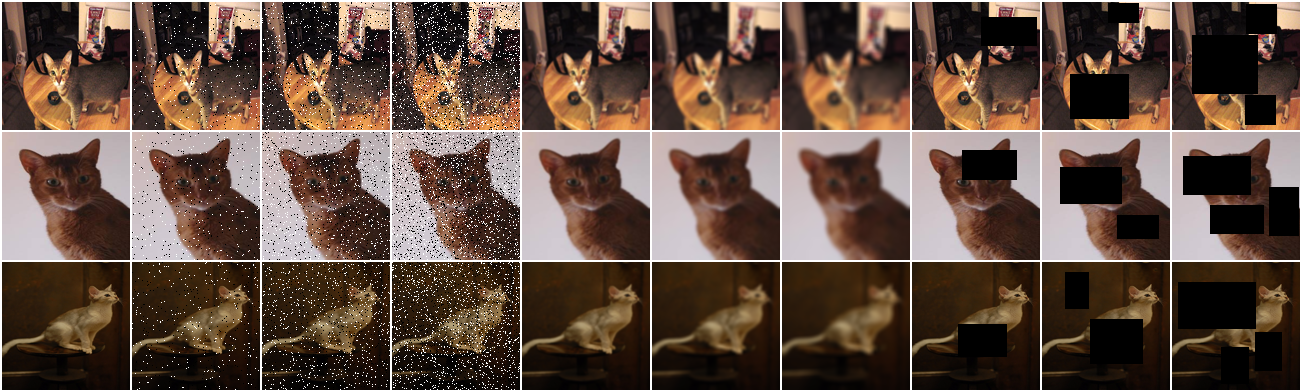
\includegraphics[width=0.95\textwidth]{corruptions.png}
\caption{Every test condition from the deterministic manifest for three test images. Columns:
clean; salt-and-pepper $p=0.03/0.08/0.15$; Gaussian blur $(3,0.7)/(5,1.5)/(7,2.5)$; occlusion with
1/2/3 rectangles covering about 10/20/35\%.}
\label{fig:corr}
\end{figure*}

%=====================================================================
\section{Task 1: Universal Denoising Autoencoder}\label{sec:t1}
%=====================================================================
\subsection{Architecture}
The encoder $E$ (Fig.~\ref{fig:dae}) is a stem convolution followed by $n$ stride-2 stages
(conv-BN-LeakyReLU $\times2$) with channels $c,2c,4c,8c$. A $1\times1$ convolution with $\tanh$ then
projects the features to a latent $z\in\mathbb{R}^{C_z\times r\times r}$. The decoder $D$ mirrors the
encoder with bilinear upsampling plus convolution, which avoids the checkerboard artefacts of transposed
convolutions~\cite{odena2016checkerboard}, and ends in a sigmoid. We chose a \emph{spatial} latent over
a fully connected vector because it keeps object layout while still forcing a large compression. With
$r\in\{8,16\}$ and $C_z\in\{4,\dots,32\}$ the latent holds 256--8,192 values, against 49,152 input
values (6$\times$--192$\times$ compression). A preliminary run showed the $8\times8$ latent saturating
near 20\,dB, so the latent resolution became an Optuna variable rather than a fixed choice.
\textbf{Summary of the selected model}: $c=32$, three stride-2 stages ($128\to64\to32\to16$, channels
32/64/128), latent $z\in\mathbb{R}^{32\times16\times16}$ (8,192 values, a 6$\times$ compression),
\textbf{496,099 learnable parameters}. The model receives only the corrupted image, never the
corruption label.

\begin{figure}[t]
\centering
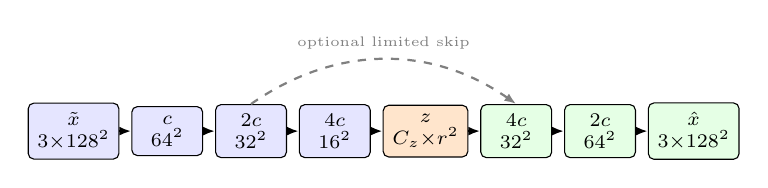
\begin{tikzpicture}[node distance=1.5mm]
\node[enc] (in) {$\tilde x$\\$3{\times}128^2$};
\node[enc, right=of in] (e1) {$c$\\$64^2$};
\node[enc, right=of e1] (e2) {$2c$\\$32^2$};
\node[enc, right=of e2] (e3) {$4c$\\$16^2$};
\node[lat, right=of e3] (z) {$z$\\$C_z{\times}r^2$};
\node[dec, right=of z] (d3) {$4c$\\$32^2$};
\node[dec, right=of d3] (d2) {$2c$\\$64^2$};
\node[dec, right=of d2] (out) {$\hat x$\\$3{\times}128^2$};
\foreach \a/\b in {in/e1,e1/e2,e2/e3,e3/z,z/d3,d3/d2,d2/out} \draw[arr] (\a) -- (\b);
\draw[arr, dashed, gray] (e2.north) to[bend left=35] node[above, font=\tiny]{optional limited skip} (d3.north);
\end{tikzpicture}
\caption{Universal DAE ($r=16$ variant shown; $r=8$ adds one $8c$ stage). Stride-2 conv stages
compress the input to a $1{\times}1$-projected spatial latent; bilinear-upsampling stages decode it. The dashed
skip is used only in the ablation.}
\label{fig:dae}
\end{figure}

\subsection{Loss and training}
The model minimises $\mathcal{L}_{\text{UDAE}} = \alpha\,\mathcal{L}_{L1}(x,\hat x) + (1-\alpha)(1-\text{SSIM}(x,\hat x))$.
We train with AdamW~\cite{loshchilov2019adamw}, a one-cycle schedule~\cite{smith2019onecycle}, mixed
precision (the loss is computed in FP32 because SSIM is numerically fragile in FP16), horizontal-flip
augmentation and early stopping on the validation objective
$J=\tfrac12\,\text{SSIM}+\tfrac12\,\text{PSNR}/40$. Dividing PSNR by 40\,dB brings it to a range
comparable with SSIM, so neither term dominates the objective.

\subsection{Hyper-parameter optimisation}
Optuna's TPE sampler (seed 42) with a median pruner searched learning rate, batch size, latent
resolution, latent channels (bottleneck dimension), encoder base channels, dropout and $\alpha$
(Table~\ref{tab:t1space}), with shortened 10-epoch trials. Of 30 trials, 23 completed and 7 were
pruned; the best (trial 23) reached $J=0.674$, up from 0.55 for the first trials (Fig.~\ref{fig:optuna1}).
fANOVA ranks learning rate, dropout and $\alpha$ as most important; latent resolution mattered once the
$8\times8$ option was shown to plateau, and every top trial used $r=16$. The selected $\alpha=0.64$
gives SSIM noticeably more weight than the brief's starting point of 0.8, consistent
with~\cite{zhao2017loss}: the structural term sharpens edges that pure L1 blurs.

\begin{figure}[t]\centering
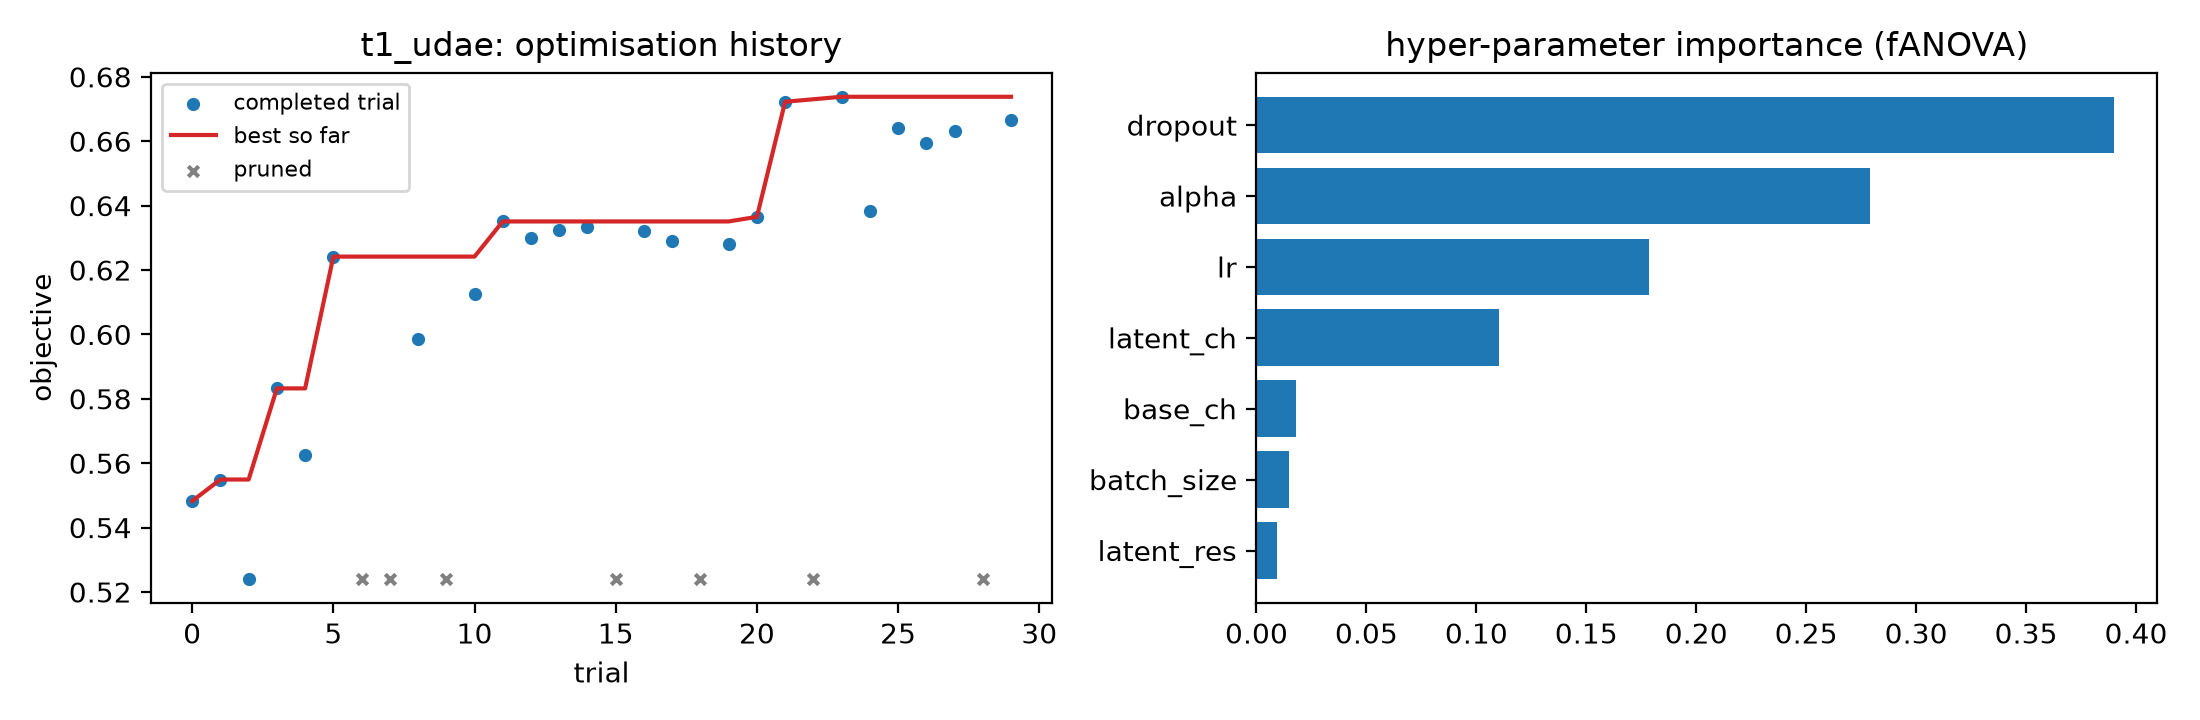
\includegraphics[width=\columnwidth]{optuna_t1_udae.png}
\caption{Task 1 Optuna study: optimisation history (left) and fANOVA importance (right).}
\label{fig:optuna1}
\end{figure}

\begin{table}[t]
\centering\caption{Task 1 Optuna search space and selected configuration.}\label{tab:t1space}
\footnotesize
\begin{tabular}{@{}lll@{}}\toprule
Parameter & Range & Selected\\\midrule
learning rate & $[10^{-4},3{\cdot}10^{-3}]$ log & $1.78{\cdot}10^{-3}$ \\
batch size & \{16, 32, 64\} & 16\\
latent resolution $r$ & \{8, 16\} & 16\\
latent channels $C_z$ & \{4, 8, 16, 32\} & 32 (8,192 values)\\
base channels $c$ & \{16, 32, 48\} & 32\\
dropout & $[0,0.3]$ & 0.079\\
$\alpha$ (L1 weight) & $[0.5,0.95]$ & 0.636\\\bottomrule
\end{tabular}
\end{table}

\subsection{Results}
The selected configuration was retrained for 60 epochs (Fig.~\ref{fig:t1curves}); validation PSNR
rose from 19\,dB to 25.3\,dB with no sign of over-fitting, because the runtime corruption pipeline
never shows the same corrupted image twice. Table~\ref{tab:t1res} reports the untouched test set.

\begin{table}[t]\centering
\caption{Task 1 test results (3,669 images $\times$ 10 conditions). ``In'' = corrupted input vs.\ clean target.}
\label{tab:t1res}\footnotesize
\begin{tabular}{@{}llrrrr@{}}\toprule
Condition & Sev. & PSNR in & PSNR out & SSIM in & SSIM out\\\midrule
Clean & -- & $\infty$ & 26.48 & 1.000 & 0.847\\
S\&P & L & 20.13 & 26.47 & 0.603 & 0.847\\
 & M & 15.87 & 26.37 & 0.339 & 0.842\\
 & H & 13.14 & 26.10 & 0.204 & 0.831\\
Blur & L & 32.34 & 26.63 & 0.944 & 0.844\\
 & M & 26.77 & 26.19 & 0.806 & 0.828\\
 & H & 24.35 & 24.59 & 0.692 & 0.736\\
Occlusion & L & 16.74 & 23.63 & 0.862 & 0.796\\
 & M & 13.30 & 21.80 & 0.727 & 0.744\\
 & H & 10.77 & 19.82 & 0.537 & 0.665\\\midrule
\multicolumn{2}{@{}l}{All corrupted} & 19.27 & \textbf{24.62} & 0.635 & \textbf{0.792}\\\bottomrule
\end{tabular}\end{table}

\begin{figure}[t]\centering
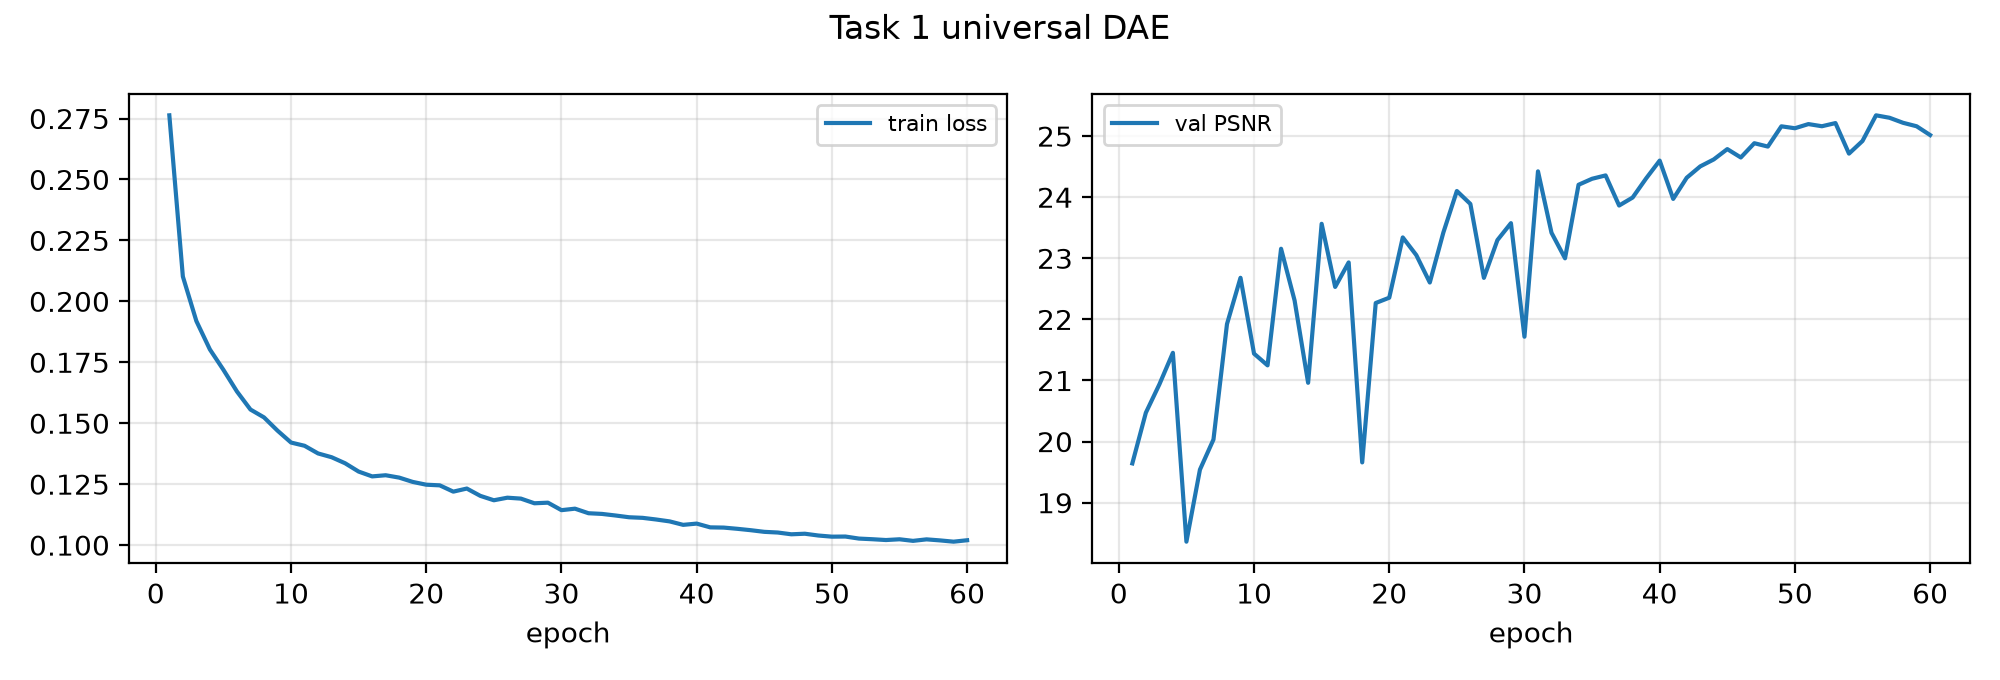
\includegraphics[width=\columnwidth]{t1_curves.png}
\caption{Task 1 final training: training loss and validation PSNR per epoch (MLflow).}
\label{fig:t1curves}
\end{figure}

\textbf{Analysis.} Salt-and-pepper is restored almost perfectly regardless of severity: output PSNR stays
at about 26.3\,dB while input PSNR falls from 20.1 to 13.1\,dB, so the gain grows to +13\,dB at
$p=0.15$. Impulse noise is spatially independent and is precisely what a bottleneck discards.
Occlusion is hardest (21.7\,dB). The model has to \emph{invent} missing content, and with no
adversarial or perceptual loss it fills the masks with smooth, locally averaged colour. The most
instructive result is the \emph{ceiling}: clean and lightly blurred inputs come out at about 26.5\,dB,
i.e.\ the autoencoder \emph{degrades} images that need no restoration (light blur: 32.3$\to$26.6\,dB).
A bottleneck of 8,192 values cannot carry all high-frequency detail of a 49,152-value image. This is
the trade-off the brief asks for: a meaningful bottleneck removes noise but also removes texture. It
directly motivates the identity bypass of Task~2 and the identity branch of Task~3.

Fig.~\ref{fig:t1ex} shows twelve representative cases (one per condition and severity, plus extras) and
Fig.~\ref{fig:t1fail} six failure cases, each with clean target, input, output and absolute-error map.
The failures fall into four groups. (1)~\emph{Hallucinated texture}: on fine grass and flowers under
heavy S\&P or blur, the decoder replaces true high-frequency texture with a mottled pattern, and the
error map lights up uniformly across the background. (2)~\emph{Occluder on a dark background}: the
network has learned that black rectangles are corruption, so it brightens them, but here the true
content \emph{is} black and the output gains a grey halo (bright border in the error map).
(3)~\emph{Large multi-rectangle occlusion}: three masks covering 35\% leave little context, and the
filled regions become flat, blurry blobs. (4)~\emph{Heavy blur on detailed scenes}: $(7,2.5)$ removes
information that cannot be recovered, and the output stays soft (SSIM 0.74).

\begin{figure}[t]\centering
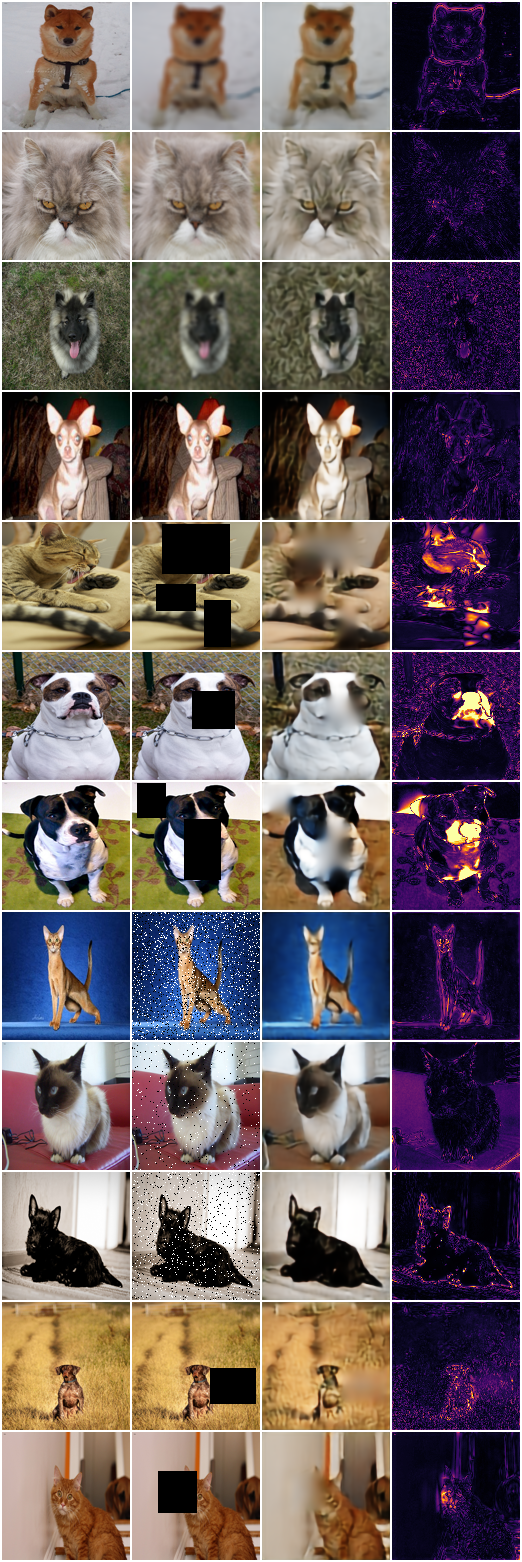
\includegraphics[width=0.85\columnwidth]{t1_examples.png}
\caption{Task 1 representative test examples. Columns: clean target, corrupted input, restoration,
$|$error$|$ map.}
\label{fig:t1ex}
\end{figure}

\begin{figure}[t]\centering
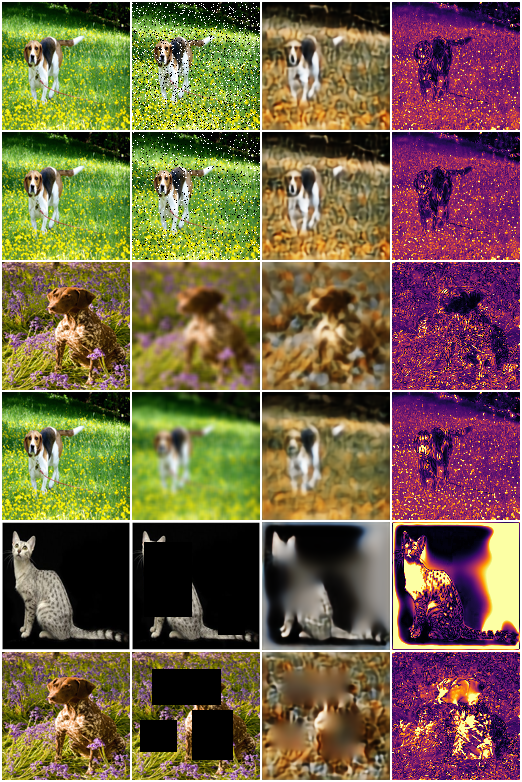
\includegraphics[width=0.85\columnwidth]{t1_failures.png}
\caption{Task 1 failure cases (lowest SSIM per corruption): hallucinated texture under S\&P and blur,
a dark-background occlusion and heavy multi-rectangle occlusion.}
\label{fig:t1fail}
\end{figure}

\textbf{Skip connections.} The final model uses \emph{no} skips. The architecture supports limited
additive skips from the deepest encoder stages (Fig.~\ref{fig:dae}, dashed), but the planned ablation
was not run before the deadline. Our expectation, from the error analysis above, is that a $32\times32$
skip would raise the clean and light-blur ceiling but would also pass occlusion masks and impulse noise
straight through. That is why skips are excluded from the bottleneck requirement.

%=====================================================================
\section{Task 2: Classifier and Hard-Routed Specialists}\label{sec:t2}
%=====================================================================
\subsection{Corruption classifier}
The classifier stacks four stages of [conv, stride-2 conv] (Fig.~\ref{fig:route}). It applies no
pooling before stride, because salt-and-pepper noise and blur are high-frequency signatures that early
pooling would average away. The head concatenates global \emph{average} and global \emph{max} pooling:
max pooling responds to sparse saturated pixels (S\&P) and to large flat black regions (occlusion).
Training uses cross-entropy on the balanced runtime batches. Optuna tuned learning rate, batch size,
channel configuration (\{16-32-64-128, 32-64-128-256, 32-64-128-128, 48-96-192-384\}), dropout
$[0,0.5]$ and weight decay $[10^{-6},10^{-2}]$ (log), maximising validation macro-F1
(Fig.~\ref{fig:optclf}). The selected classifier has \textbf{1,239,396 parameters}.

\begin{figure}[t]\centering
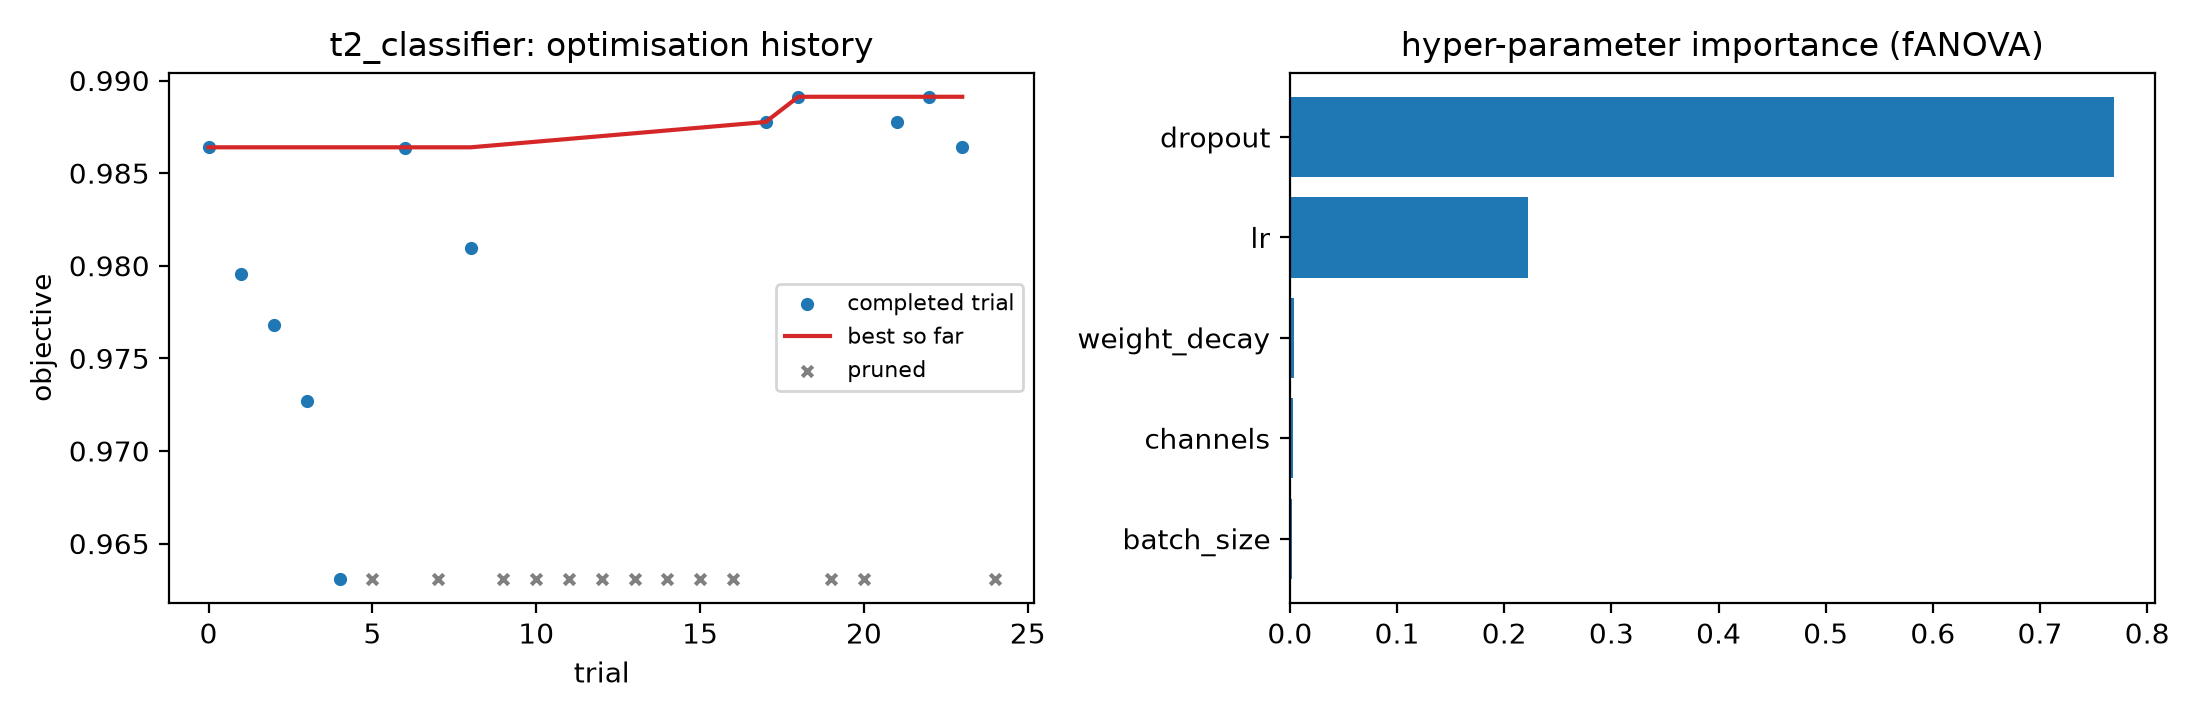
\includegraphics[width=\columnwidth]{optuna_t2_classifier.png}
\caption{Classifier Optuna study (25 trials; 12 completed, 13 pruned).}\label{fig:optclf}
\end{figure}

\subsection{Specialists}
Three autoencoders with the Task~1 architecture are trained independently, each only on its own
corruption with the clean image as target. To keep the cost feasible, a single \emph{shared} Optuna
study selects the common architecture and optimiser settings (learning rate, latent size, channels,
batch size, $\alpha$) by maximising the mean validation objective of the three specialists. The three
final models are then trained from scratch with independent parameters.

\textbf{Short-horizon bias (a difficulty we hit).} The first shared study used 6-epoch trials (15
trials, 10 completed). It selected a tiny 4-channel latent (1,024 values), which converges quickly
but plateaus: after full training the specialists reached only 24.3/24.3/20.7\,dB on S\&P/blur/occlusion
validation, about 2\,dB \emph{below} the universal model, even though each specialist faces an easier
problem. This is the known short-horizon bias of multi-fidelity tuning: short trials reward fast early
progress rather than final quality. We therefore ran a second study with 15-epoch trials,
warm-started with the Task~1 configuration. Its best trial (the warm start, 32-channel latent) scored
0.689, against 0.585 for the short study (Fig.~\ref{fig:optspec}). All three specialists were then
retrained with this configuration (20 epochs each, compute-limited). Validation PSNR/SSIM improved from
24.3/0.74, 24.3/0.73 and 20.7/0.65 to \textbf{26.1/0.82, 25.9/0.81 and 21.3/0.71} for S\&P, blur and
occlusion. The evidence from the second study therefore fixed a 1.5--2\,dB deficit that the first study
had introduced. Each specialist uses the same architecture as Task~1 ($c=32$, 8,192-value latent,
\textbf{496,099 parameters each}, 1.49\,M in total) with independently trained weights. Its training
curves are shown in Fig.~\ref{fig:speccurves}, and its per-severity test performance is the oracle
column of Table~\ref{tab:t2sev}.

\begin{figure}[t]\centering
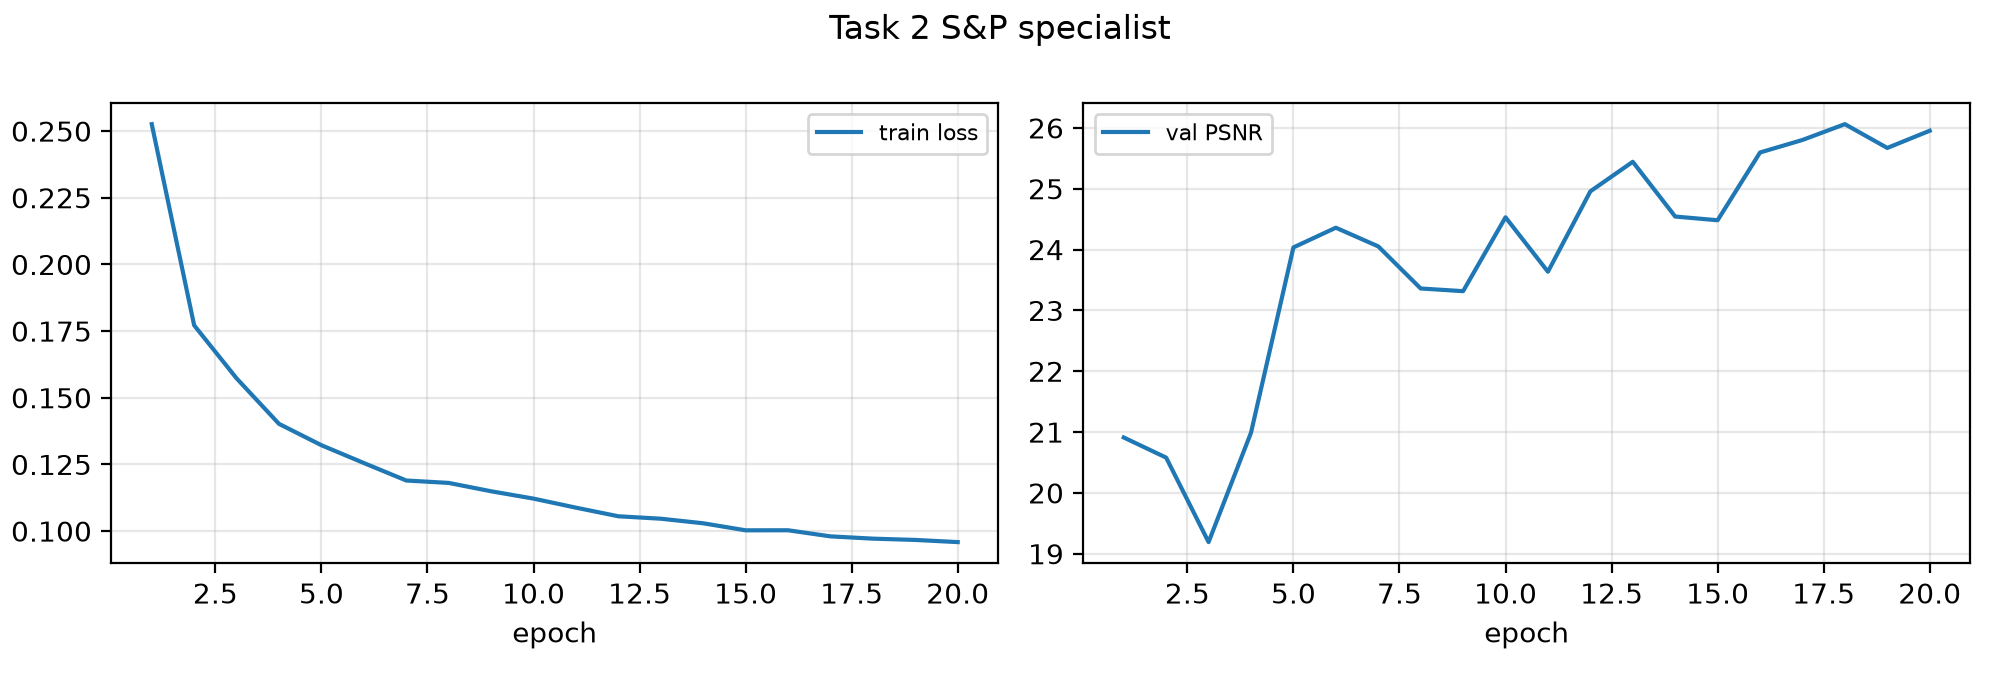
\includegraphics[width=\columnwidth]{t2_spec_sp_curves.png}\\
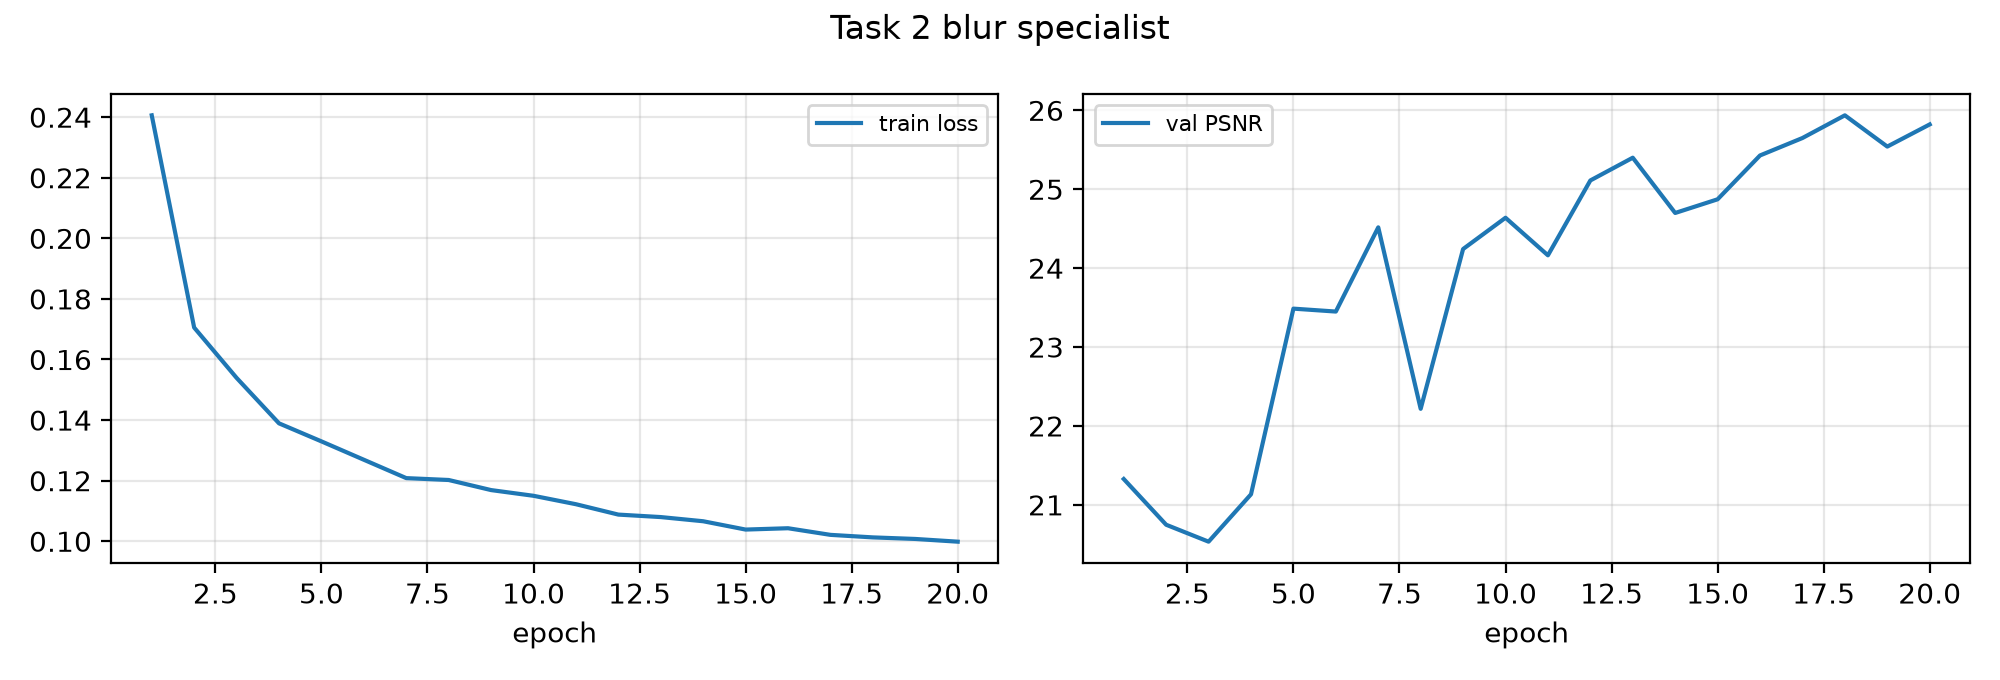
\includegraphics[width=\columnwidth]{t2_spec_blur_curves.png}\\
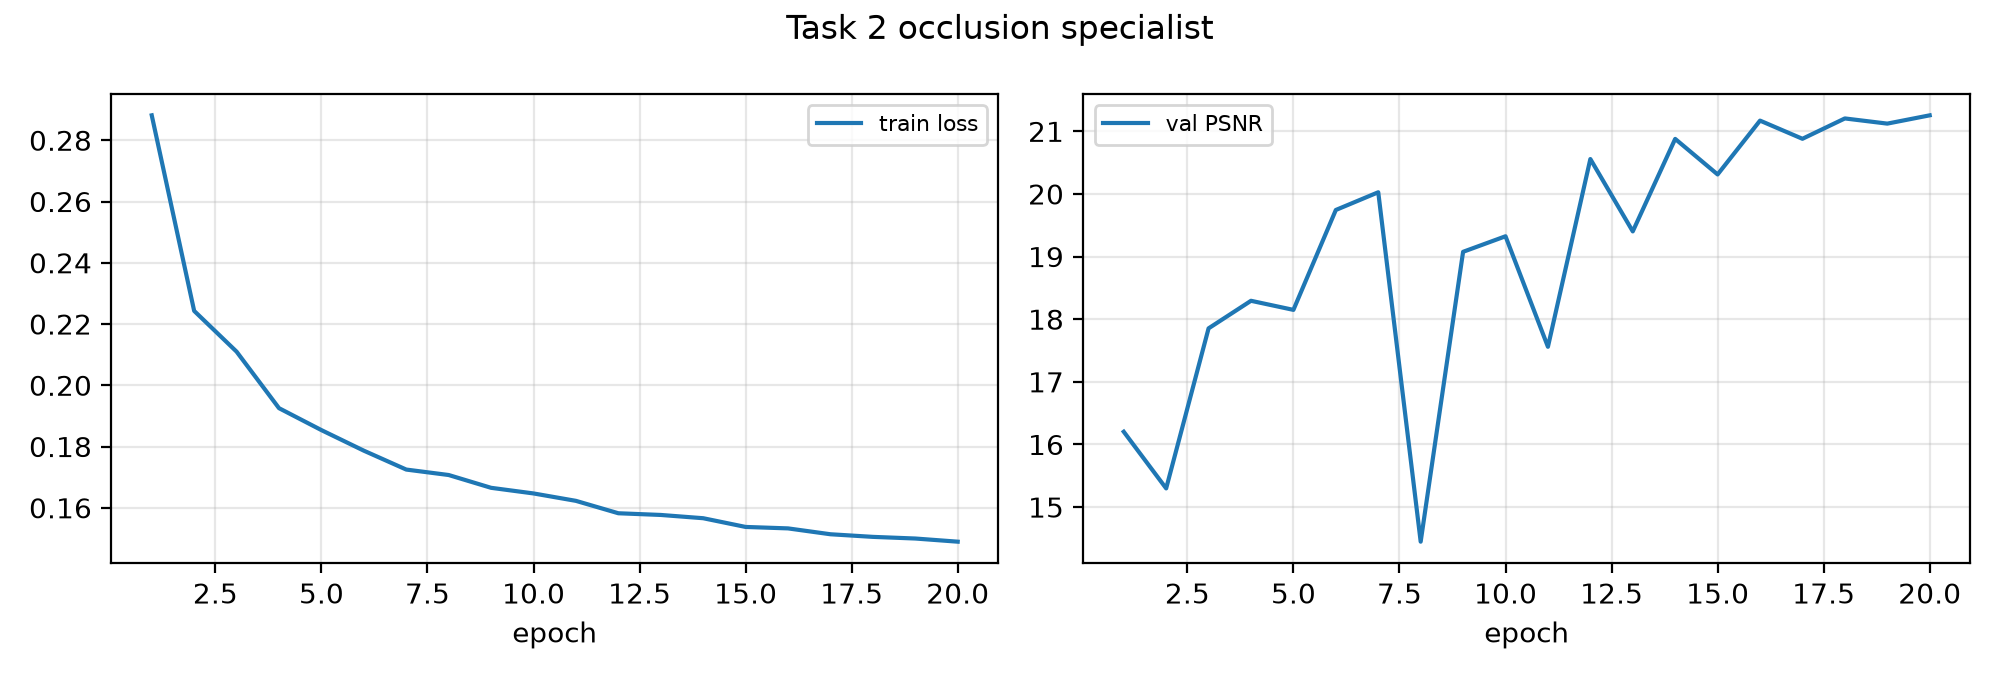
\includegraphics[width=\columnwidth]{t2_spec_occ_curves.png}
\caption{Training loss and validation PSNR of the S\&P (top), blur (middle) and occlusion (bottom)
specialists.}\label{fig:speccurves}
\end{figure}

\begin{figure}[t]\centering
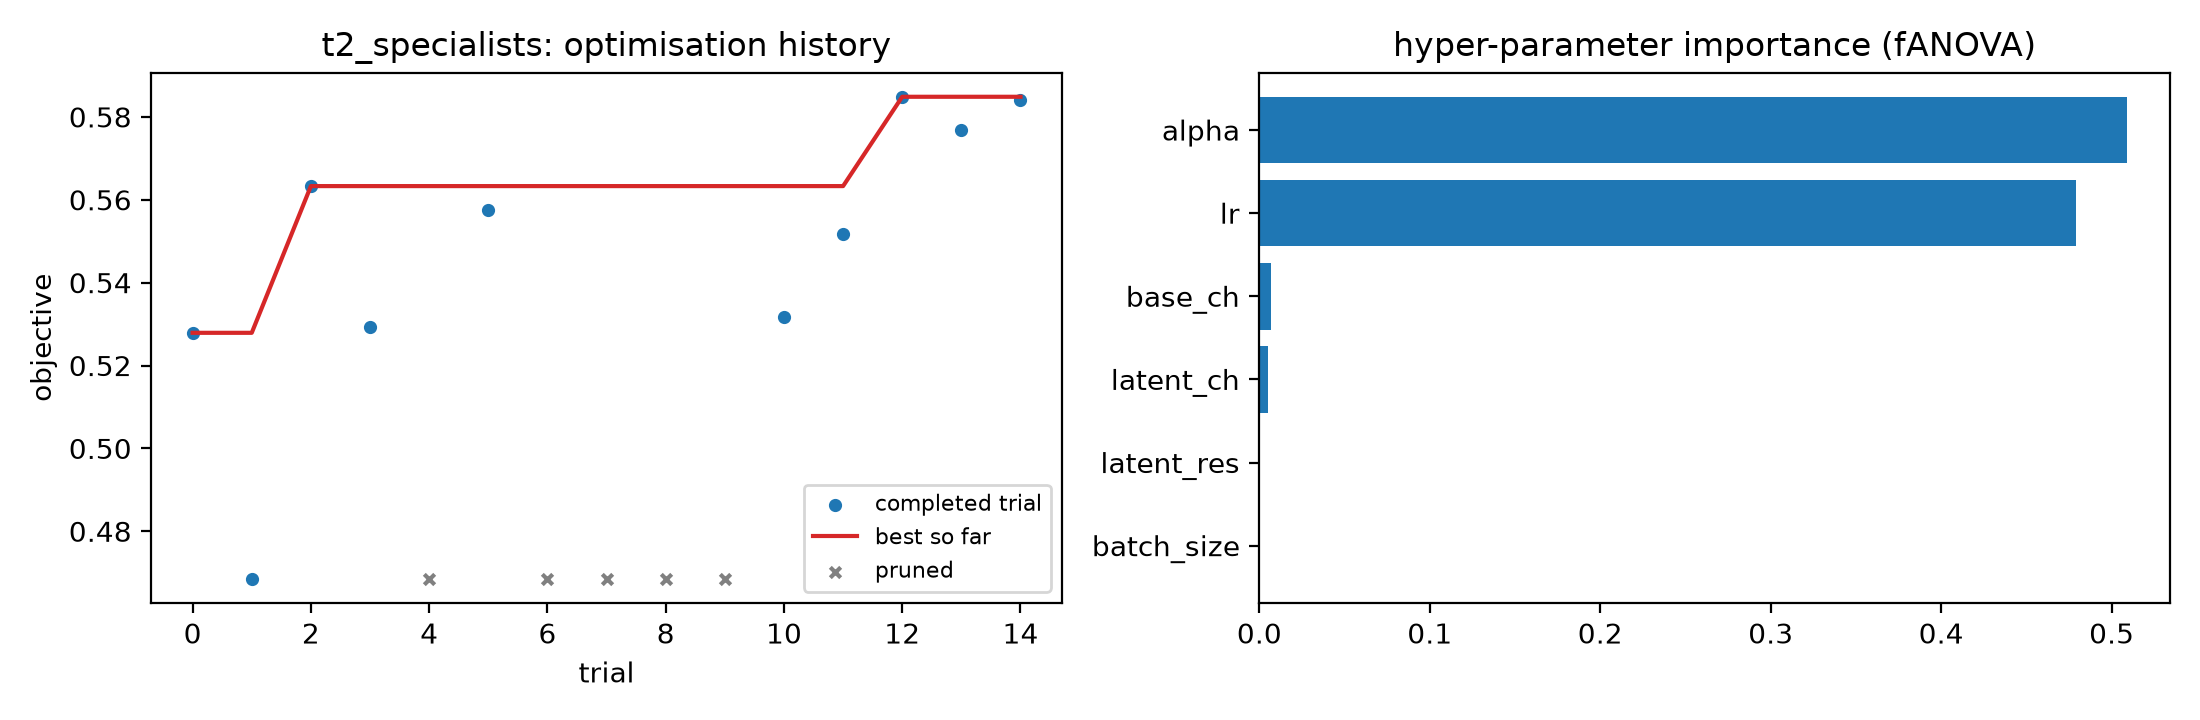
\includegraphics[width=\columnwidth]{optuna_t2_specialists.png}\\
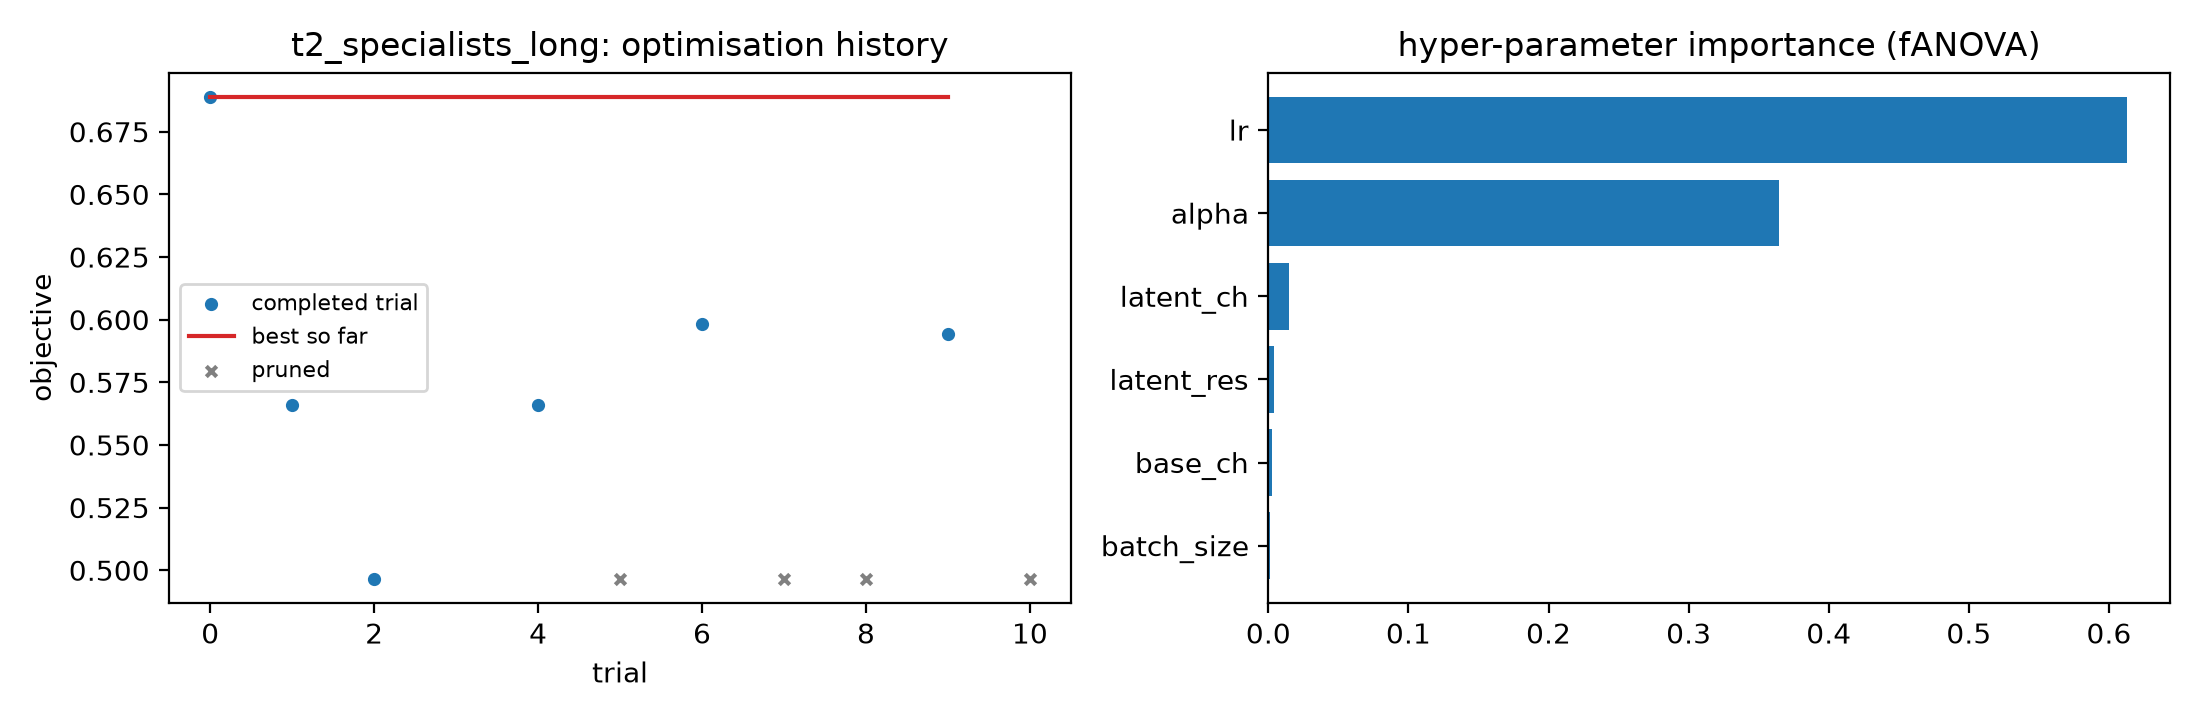
\includegraphics[width=\columnwidth]{optuna_t2_specialists_long.png}
\caption{Shared specialist studies: 6-epoch trials (top) versus 15-epoch trials, warm-started (bottom).}
\label{fig:optspec}
\end{figure}

\subsection{Hard routing}
At inference the class $r=\arg\max_k p_k$ selects $\hat x=\tilde x$ (identity bypass for \emph{clean}) or
$A_r(\tilde x)$. We evaluate \emph{oracle} routing (label from the test manifest), which measures
specialist capability, and \emph{predicted} routing, which measures the deployed system.

\begin{figure}[t]
\centering
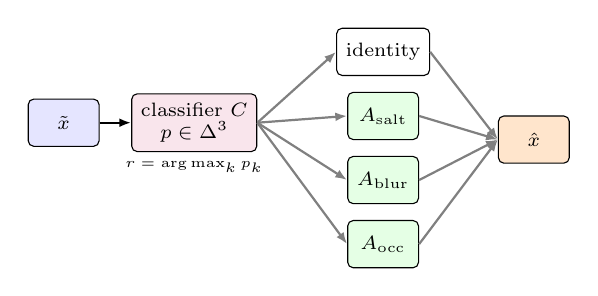
\begin{tikzpicture}[node distance=2mm and 4mm]
\node[enc] (x) {$\tilde x$};
\node[blk, fill=purple!10, right=of x] (c) {classifier $C$\\$p\in\Delta^3$};
\node[blk, right=10mm of c, yshift=9mm] (i) {identity};
\node[dec, below=of i] (a1) {$A_{\text{salt}}$};
\node[dec, below=of a1] (a2) {$A_{\text{blur}}$};
\node[dec, below=of a2] (a3) {$A_{\text{occ}}$};
\node[lat, right=10mm of a1, yshift=-3mm] (o) {$\hat x$};
\draw[arr] (x) -- (c);
\foreach \n in {i,a1,a2,a3} {\draw[arr, gray] (c.east) -- (\n.west); \draw[arr, gray] (\n.east) -- (o.west);}
\node[font=\tiny, below=0mm of c] {$r=\arg\max_k p_k$};
\end{tikzpicture}
\caption{Hard routing: exactly one branch is executed per image.}
\label{fig:route}
\end{figure}

\subsection{Results}
\textbf{Classifier.} Its Optuna study (25 trials, 12 completed, 13 pruned) selected learning rate
$2.7{\cdot}10^{-4}$, batch 32, channels 32-64-128-256, dropout 0.07 and weight decay $1.7{\cdot}10^{-4}$
(validation macro-F1 0.989 in 6 epochs). After 40 epochs it reached 99.7\% validation accuracy. On all
36,690 test cases it achieves \textbf{99.82\% accuracy}, macro precision 0.998, macro recall 0.996 and
\textbf{macro-F1 0.997} (Table~\ref{tab:clf}, Fig.~\ref{fig:cm}). S\&P is perfect: isolated saturated
pixels are unmistakable to the max-pooling branch. Nearly all errors are \emph{clean} images predicted
as occlusion (0.71\%) or blur (0.84\%); low-severity blur and occlusion are the only corrupted classes
below 100\%.

\begin{table}[t]\centering\caption{Task 2 classifier on the test manifest.}\label{tab:clf}\footnotesize
\begin{tabular}{@{}lrrrr@{}}\toprule
Class & Precision & Recall & F1 & Support\\\midrule
Clean & 0.998 & 0.984 & 0.991 & 3,669\\
Salt \& pepper & 1.000 & 1.000 & 1.000 & 11,007\\
Blur & 0.997 & 1.000 & 0.998 & 11,007\\
Occlusion & 0.998 & 1.000 & 0.999 & 11,007\\\midrule
Macro avg & 0.998 & 0.996 & 0.997 & 36,690\\\bottomrule
\end{tabular}\end{table}

\begin{figure}[t]\centering
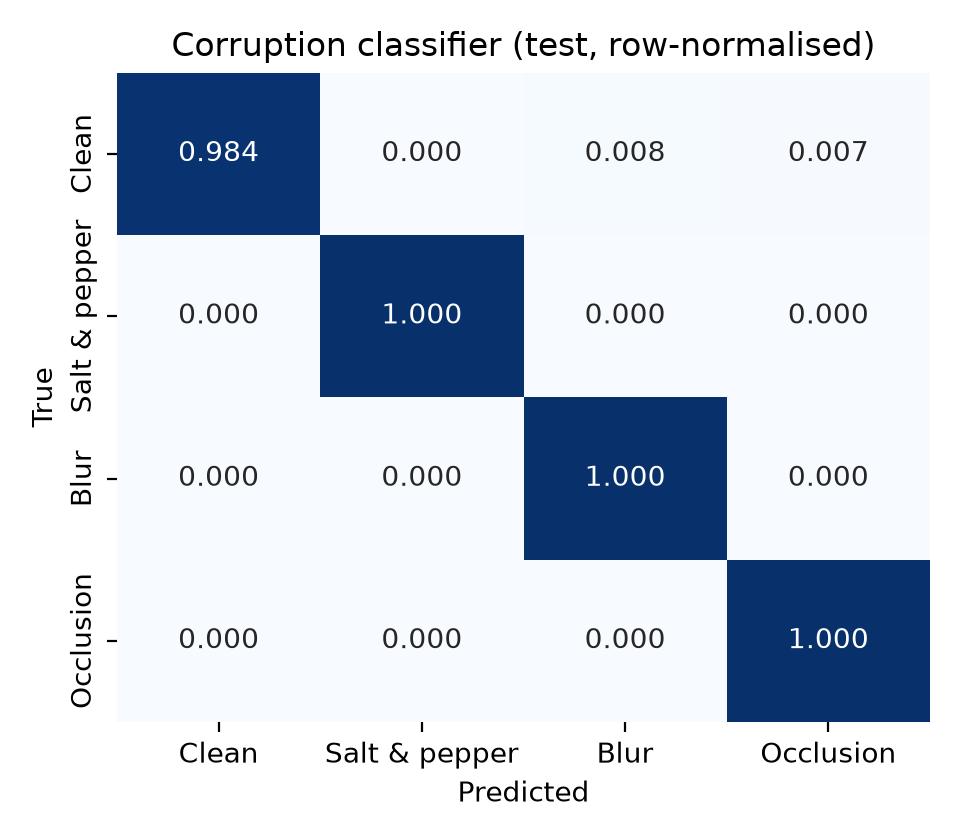
\includegraphics[width=0.75\columnwidth]{t2_confusion.png}
\caption{Row-normalised confusion matrix of the corruption classifier (test).}
\label{fig:cm}
\end{figure}

\textbf{Routing.} Because the classifier is so accurate, predicted and oracle routing differ by at most
0.02\,dB on every corrupted cell; overall corrupted PSNR is 24.31 (predicted) vs.\ 24.31\,dB (oracle),
SSIM 0.778 (Table~\ref{tab:compare}). Clean inputs pass through the identity bypass unchanged in
98.4\% of cases (clean SSIM 0.997 vs.\ 0.847 for Task~1), which removes Task~1's main weakness. On
corrupted inputs Task~2 is slightly \emph{below} Task~1 (24.3 vs.\ 24.6\,dB). Since the oracle row is
identical, this is not a routing problem. The specialists simply received 20 training epochs against
Task~1's 60, which shows that a hard-routed system is only as good as its experts.

\begin{table}[t]\centering
\caption{Task 2 hard routing by corruption and severity: oracle (true label selects the expert, i.e.\
per-specialist performance) vs.\ predicted (classifier selects). PSNR\,dB / SSIM; last column =
fraction of misrouted images.}\label{tab:t2sev}\footnotesize
\begin{tabular}{@{}llccr@{}}\toprule
Condition & Sev. & Oracle & Predicted & Misr.\\\midrule
Clean & -- & $\infty$ / 1.000 & 98.8 / 0.997 & 1.55\%\\
S\&P & L & 25.98 / 0.828 & 25.98 / 0.828 & 0\%\\
 & M & 25.92 / 0.826 & 25.92 / 0.826 & 0\%\\
 & H & 25.77 / 0.819 & 25.77 / 0.819 & 0\%\\
Blur & L & 25.76 / 0.824 & 25.76 / 0.824 & 0.11\%\\
 & M & 25.91 / 0.819 & 25.91 / 0.819 & 0\%\\
 & H & 24.66 / 0.745 & 24.66 / 0.745 & 0\%\\
Occlusion & L & 23.18 / 0.767 & 23.19 / 0.767 & 0.14\%\\
 & M & 21.66 / 0.721 & 21.66 / 0.721 & 0\%\\
 & H & 19.92 / 0.652 & 19.92 / 0.652 & 0\%\\\bottomrule
\end{tabular}\end{table}

\textbf{When specialists help.} Compared with Task~1 (Table~\ref{tab:t1res}), the specialists are
slightly behind at low and medium severity (by 0.1--0.9\,dB) but level or ahead at high severity (blur
24.66 vs.\ 24.59\,dB; occlusion 19.92 vs.\ 19.82\,dB). The clear win is on clean and nearly clean inputs: the identity
bypass returns them untouched, whereas the universal model caps them at 26.5\,dB. Specialists fail when
the router fails, and when an input contains a corruption they never saw (the mixed test in
Sec.~\ref{sec:t3}).

\textbf{Classifier-induced failures} (Fig.~\ref{fig:misroute}). The worst routing errors are all
\emph{clean} images with large uniform black regions: black studio backgrounds, letterbox bars, a dark
car interior. The classifier sees large zero-valued areas and predicts occlusion. The occlusion expert,
trained only to fill black rectangles, then ``inpaints'' the legitimate black background with grey or
white and blurs the subject, so PSNR collapses from $\infty$ (identity) to 12--16\,dB. Saturated,
colourful clean images (a purple backdrop, rainbow balloons) are occasionally routed to blur and
suffer colour shifts. These cases show the fragility of a hard decision: a 1.6\% error rate on
clean images produces the largest per-image losses in the whole task. A soft gate that hedges between
the identity and an expert, or an explicit ``uncertain'' fallback to identity, would bound the damage.

\begin{figure}[t]\centering
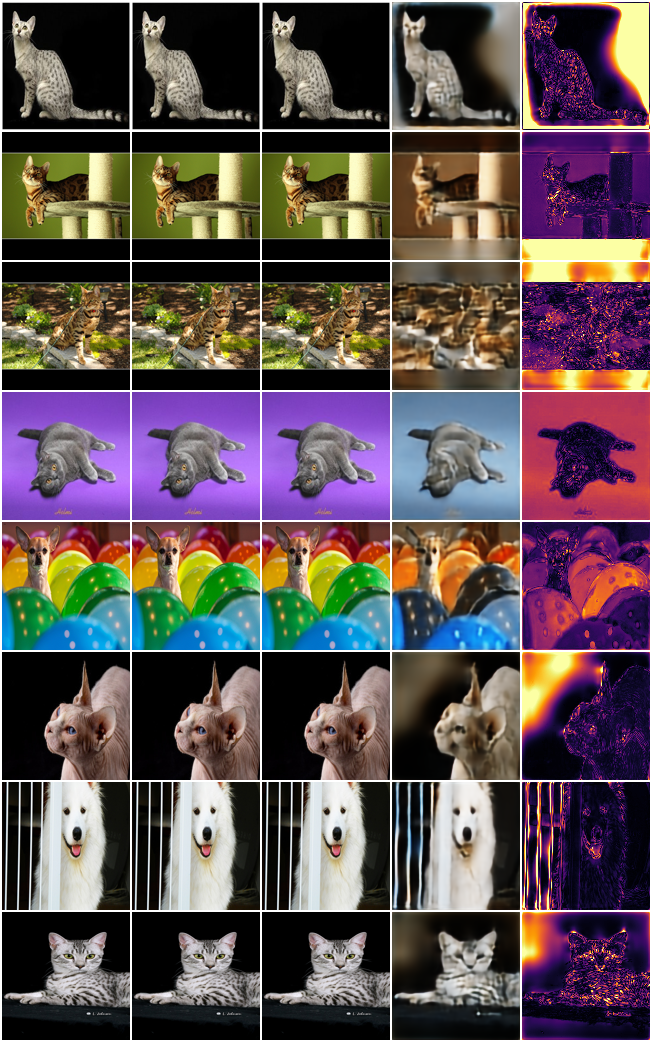
\includegraphics[width=0.85\columnwidth]{t2_misrouted.png}
\caption{Misrouting failures. Columns: clean, input (clean), oracle output (identity), predicted-route
output, error. Uniform black backgrounds are mistaken for occlusion.}
\label{fig:misroute}
\end{figure}

%=====================================================================
\section{Task 3: Soft Mixture-of-Experts}\label{sec:t3}
%=====================================================================
\subsection{Model}
The gate $G$ is the Task~2 classifier, and its logits give $w=\text{softmax}(G(\tilde x)/\tau)$ over
[identity, S\&P, blur, occlusion]. The output is $\hat x = w_0\tilde x + \sum_{k=1}^{3} w_k A_k(\tilde x)$.
Branch~0 matches the classifier's \emph{clean} class, so the initial gate is already meaningful. The
whole pipeline, including the identity branch and the weighted sum, is exported as \emph{one} ONNX
graph with outputs (restored, weights, logits). In total it has \textbf{2,727,693 parameters}: the gate
(1.24\,M) plus three experts (3$\times$0.50\,M). Fig.~\ref{fig:moe} shows the architecture.

\begin{figure}[t]\centering
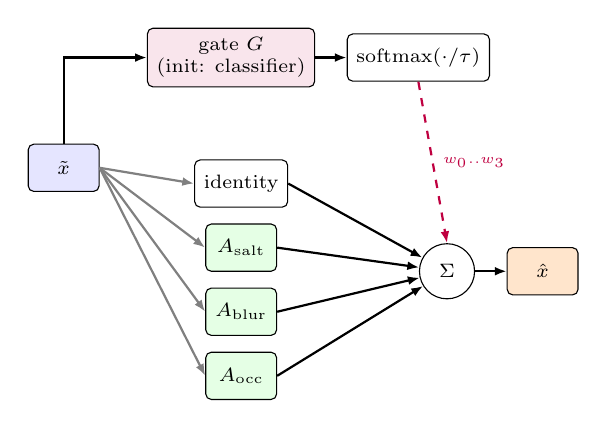
\begin{tikzpicture}[node distance=2mm and 5mm]
\node[enc] (x) {$\tilde x$};
\node[blk, fill=purple!10, right=6mm of x, yshift=14mm] (g) {gate $G$\\(init: classifier)};
\node[blk, right=4mm of g] (sm) {softmax$(\cdot/\tau)$};
\node[blk, right=12mm of x, yshift=-2mm] (i) {identity};
\node[dec, below=of i] (a1) {$A_{\text{salt}}$};
\node[dec, below=of a1] (a2) {$A_{\text{blur}}$};
\node[dec, below=of a2] (a3) {$A_{\text{occ}}$};
\node[blk, circle, minimum width=7mm, right=18mm of a1, yshift=-3mm] (sum) {$\Sigma$};
\node[lat, right=4mm of sum] (o) {$\hat x$};
\draw[arr] (x) |- (g);
\draw[arr] (g) -- (sm);
\foreach \n in {i,a1,a2,a3} {\draw[arr, gray] (x.east) -- (\n.west); \draw[arr] (\n.east) -- (sum);}
\draw[arr, dashed, purple] (sm.south) -- node[right, font=\tiny]{$w_0..w_3$} (sum.north);
\draw[arr] (sum) -- (o);
\end{tikzpicture}
\caption{Soft mixture of experts: all four branches run, and their outputs are mixed by the
temperature-scaled gate weights, $\hat x=w_0\tilde x+\sum_k w_kA_k(\tilde x)$. The whole graph is
differentiable and is exported to ONNX as a single model.}
\label{fig:moe}
\end{figure}

\subsection{Training}
Joint training does not start from random components. The gate and experts are loaded from Task~2.
(1)~\emph{Warm-up}: the experts are frozen (parameters and BatchNorm statistics) and only the gate
trains for one epoch (two in the original design), adapting to the temperature and to the reconstruction signal. (2)~\emph{Joint
fine-tuning}: all parameters train at a smaller learning rate. The loss is
$\mathcal{L}_{\text{MoE}}=\lambda_1\mathcal{L}_{L1}+\lambda_s(1-\text{SSIM})+\lambda_c\mathcal{L}_{CE}+\lambda_b\mathcal{L}_{\text{balance}}$,
where $\mathcal{L}_{CE}=-\log w_y$ is computed on the temperature-scaled distribution that is actually
used for mixing, and $\mathcal{L}_{\text{balance}}=\sum_k(\bar w_k-\frac14)^2$. Because every batch is
exactly class-balanced, perfect routing gives $\bar w_k=\frac14$. The balance term therefore penalises
\emph{collapse} without penalising correct specialisation. A per-sample entropy bonus, by contrast,
would discourage confident correct routing, which is why we rejected it. This is the same motivation as
the load-balancing losses of~\cite{shazeer2017moe,fedus2022switch}.

\subsection{Optuna}
The study searches the joint learning rate, $\tau$, $\lambda_c$, $\lambda_b$ and $\lambda_1$ (with
$\lambda_s=1-\lambda_1$). A custom pruning rule stops any trial in which some branch's mean
validation weight falls below 0.02 (\emph{routing collapse}), in addition to median pruning.

\subsection{Selected configuration}
Four trials (compute-limited; 1 warm-up epoch and 2 joint epochs each) all completed without routing
collapse. The clearest effect was temperature: the two sharp gates ($\tau=0.34$ and $0.60$) scored
0.905 and 0.900, against 0.883 and 0.847 for $\tau\approx2.7$. With a 99.8\%-accurate classifier, decisive
routing pays off. Selected: $\tau=0.34$, $\lambda_c=0.43$, $\lambda_b=0.006$, $\lambda_1=0.82$. Before
any fine-tuning, the classifier-initialised gate already routed 99.7\% of validation images correctly
with balanced mean weights (0.23--0.26), which confirms that initialising from Task~2 avoids a
random-gate collapse. The final model was trained with 1 warm-up epoch and 6 joint epochs at
$\text{lr}=1.7{\cdot}10^{-5}$ (Fig.~\ref{fig:t3curves}). Validation PSNR rose steadily, and the
minimum mean branch weight never fell below the collapse threshold.

\begin{figure}[t]\centering
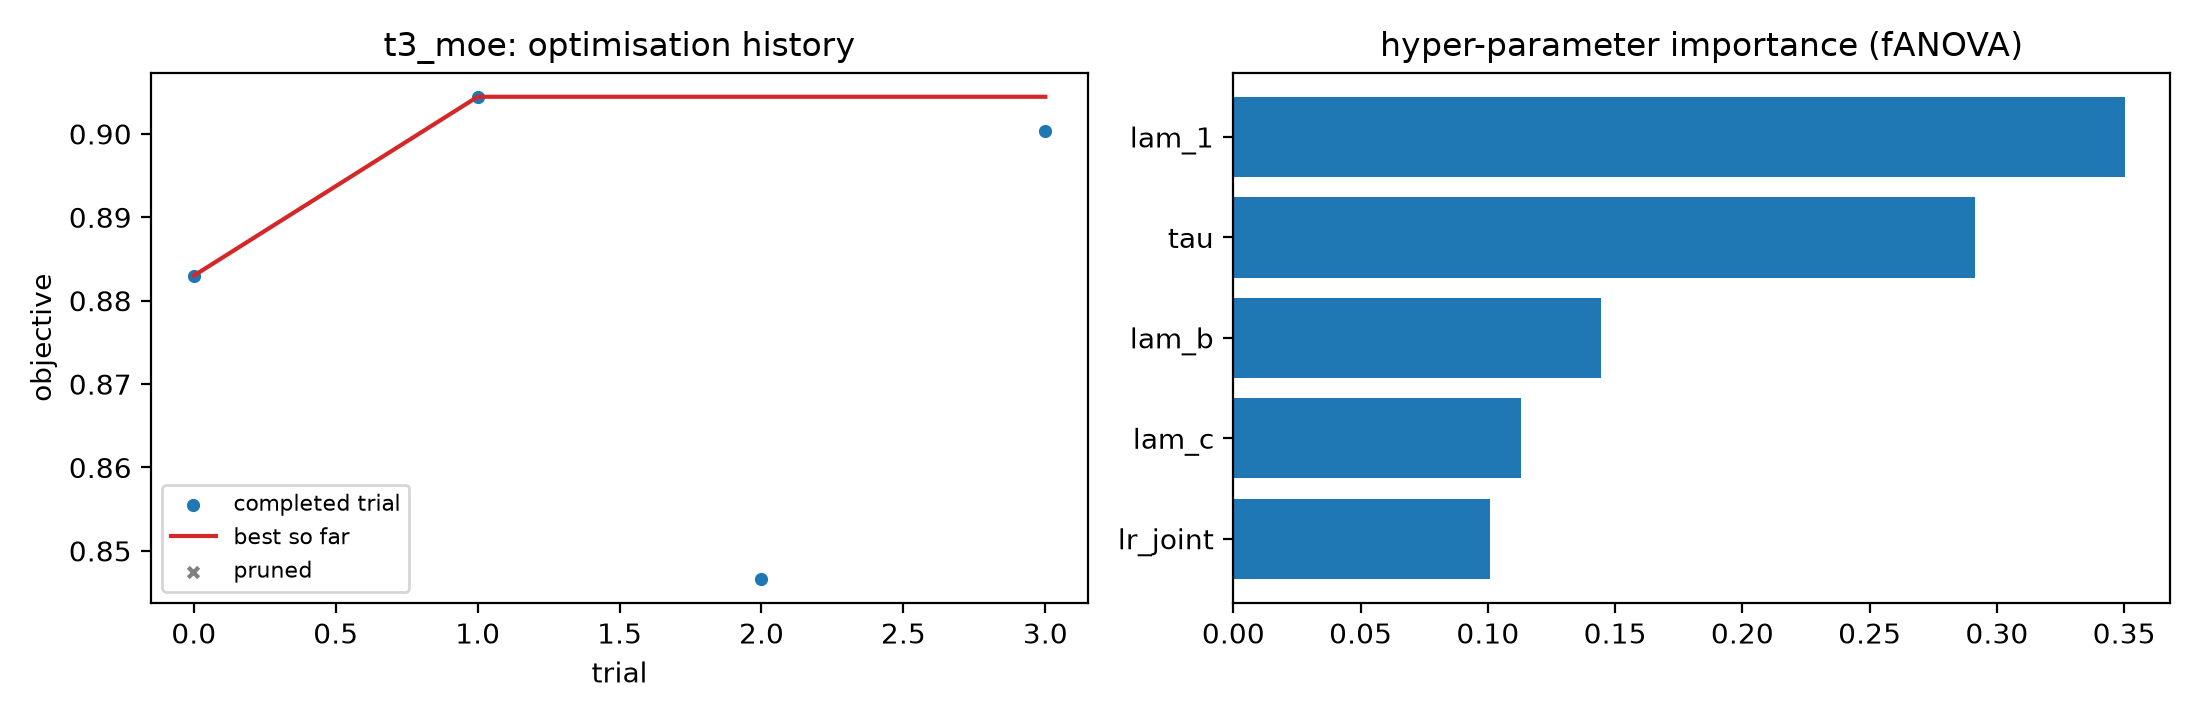
\includegraphics[width=\columnwidth]{optuna_t3_moe.png}\\
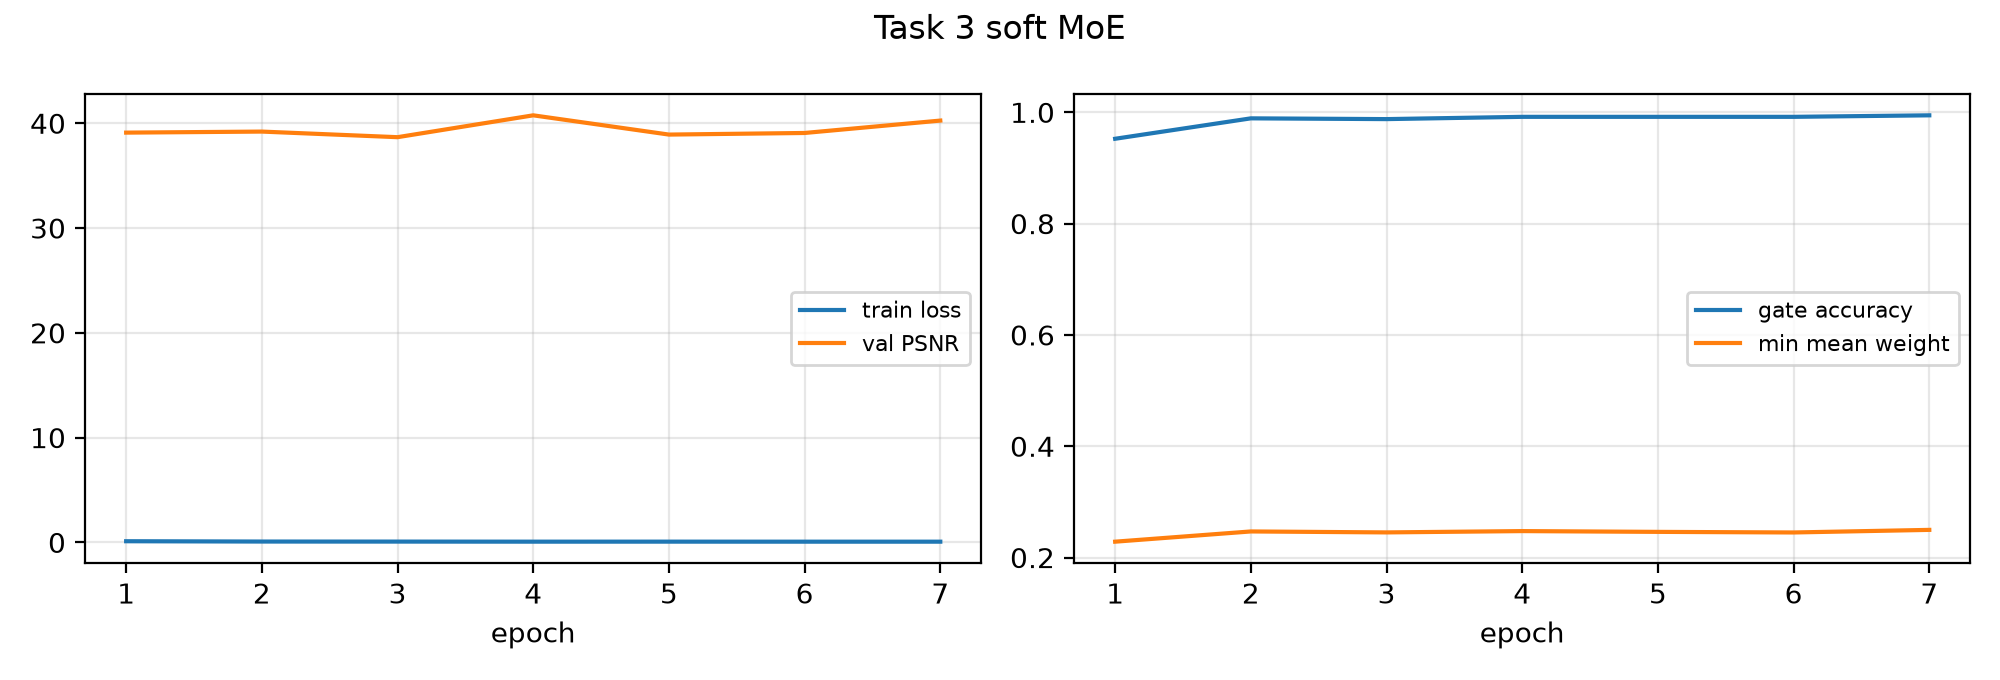
\includegraphics[width=\columnwidth]{t3_curves.png}
\caption{Task 3: Optuna study (top) and final training curves (bottom): loss, validation PSNR, gate
accuracy and minimum mean branch weight.}\label{fig:t3curves}
\end{figure}

\subsection{Results}
Table~\ref{tab:compare} compares the three restoration systems on the test manifest.

\begin{table}[t]\centering
\caption{Restoration methods on the test set (PSNR\,dB / SSIM).}\label{tab:compare}\footnotesize
\begin{tabular}{@{}lccc@{}}\toprule
Condition & T1 universal & T2 hard (pred.) & T3 soft MoE\\\midrule
Clean & 26.48 / 0.847 & $\approx\infty$ / 0.997 & $\approx\infty$ / 0.998\\
Salt \& pepper & \textbf{26.31} / \textbf{0.840} & 25.89 / 0.824 & 25.61 / 0.819\\
Blur & \textbf{25.80} / \textbf{0.803} & 25.44 / 0.796 & 25.40 / 0.792\\
Occlusion & \textbf{21.75} / \textbf{0.735} & 21.59 / 0.713 & 21.47 / 0.703\\\midrule
All corrupted & \textbf{24.62} / \textbf{0.792} & 24.31 / 0.778 & 24.16 / 0.771\\\bottomrule
\end{tabular}\end{table}

\begin{table}[t]\centering
\caption{PSNR (dB) by corruption and severity for all restoration systems.}\label{tab:sevcmp}\footnotesize
\begin{tabular}{@{}llrrrr@{}}\toprule
Cond. & Sev. & T1 & T2 oracle & T2 pred. & T3 MoE\\\midrule
S\&P & L & \textbf{26.47} & 25.98 & 25.98 & 25.55\\
 & M & \textbf{26.37} & 25.92 & 25.92 & 25.68\\
 & H & \textbf{26.10} & 25.77 & 25.77 & 25.60\\
Blur & L & \textbf{26.63} & 25.76 & 25.76 & 25.70\\
 & M & \textbf{26.19} & 25.91 & 25.91 & 25.88\\
 & H & 24.59 & \textbf{24.66} & \textbf{24.66} & 24.63\\
Occl. & L & \textbf{23.63} & 23.18 & 23.19 & 23.14\\
 & M & \textbf{21.80} & 21.66 & 21.66 & 21.52\\
 & H & 19.82 & \textbf{19.92} & \textbf{19.92} & 19.75\\\bottomrule
\end{tabular}\end{table}

Table~\ref{tab:sevcmp} breaks the comparison down by severity. The ordering is the same everywhere:
Task~1 is ahead by 0.1--0.9\,dB at low and medium severity, while the specialist-based systems catch up
or win at high severity. This is consistent with the specialists' shorter training: they are only
slightly behind where the problem is easy. The soft MoE is within 0.1--0.4\,dB of hard routing in every
cell, as expected from its near-hard gate.

\textbf{Gate behaviour.} The mean-weight heatmap (Fig.~\ref{fig:heat}) is almost perfectly diagonal:
at medium and high severity the correct branch receives $\ge$0.999 of the weight, and 99.0\% of all test
images have one branch with $w\ge0.9$. The top-weighted branch matches the true corruption for 99.6\% of
images. \emph{No expert is inactive}: mean weights are 0.30/0.30/0.30 for the experts and 0.10 for the
identity, which matches the 3:3:3:1 class mix of the test manifest. \emph{No expert dominates unrelated
inputs}: the mean weight a branch receives on inputs it is not responsible for is at most 0.005. The
only real hedging happens at \emph{low severity} (Fig.~\ref{fig:dist}): faint blur, sparse noise
or a small occluder produce near 50/50 splits between the identity and the matching expert. That is
the sensible output when the corruption barely changes the image.

\textbf{Mixed corruptions.} On 300 test images with two simultaneous medium corruptions, which none of
the models saw in training, the universal DAE is best on every pair (blur+occlusion 21.9, S\&P+blur
22.3, S\&P+occlusion 21.6\,dB). For S\&P+occlusion, the gate splits 0.84/0.16 between the S\&P and
occlusion experts, and this blend beats hard routing (14.5 vs.\ 13.6\,dB). It still falls far short
of the universal model, because each expert has only seen one corruption and treats the other as
signal.

\textbf{Interpretation.} With a near-perfect classifier and a strong CE term, joint fine-tuning keeps
the gate close to its initialisation. The soft MoE then behaves as a smoothed hard router: it matches
hard routing in distribution, hedges where it should, and is fully differentiable, but it cannot exceed
the quality of its experts. A longer joint stage with a smaller $\lambda_c$, or experts trained on
mixtures, would be needed to exploit the soft combination.

\begin{figure}[t]\centering
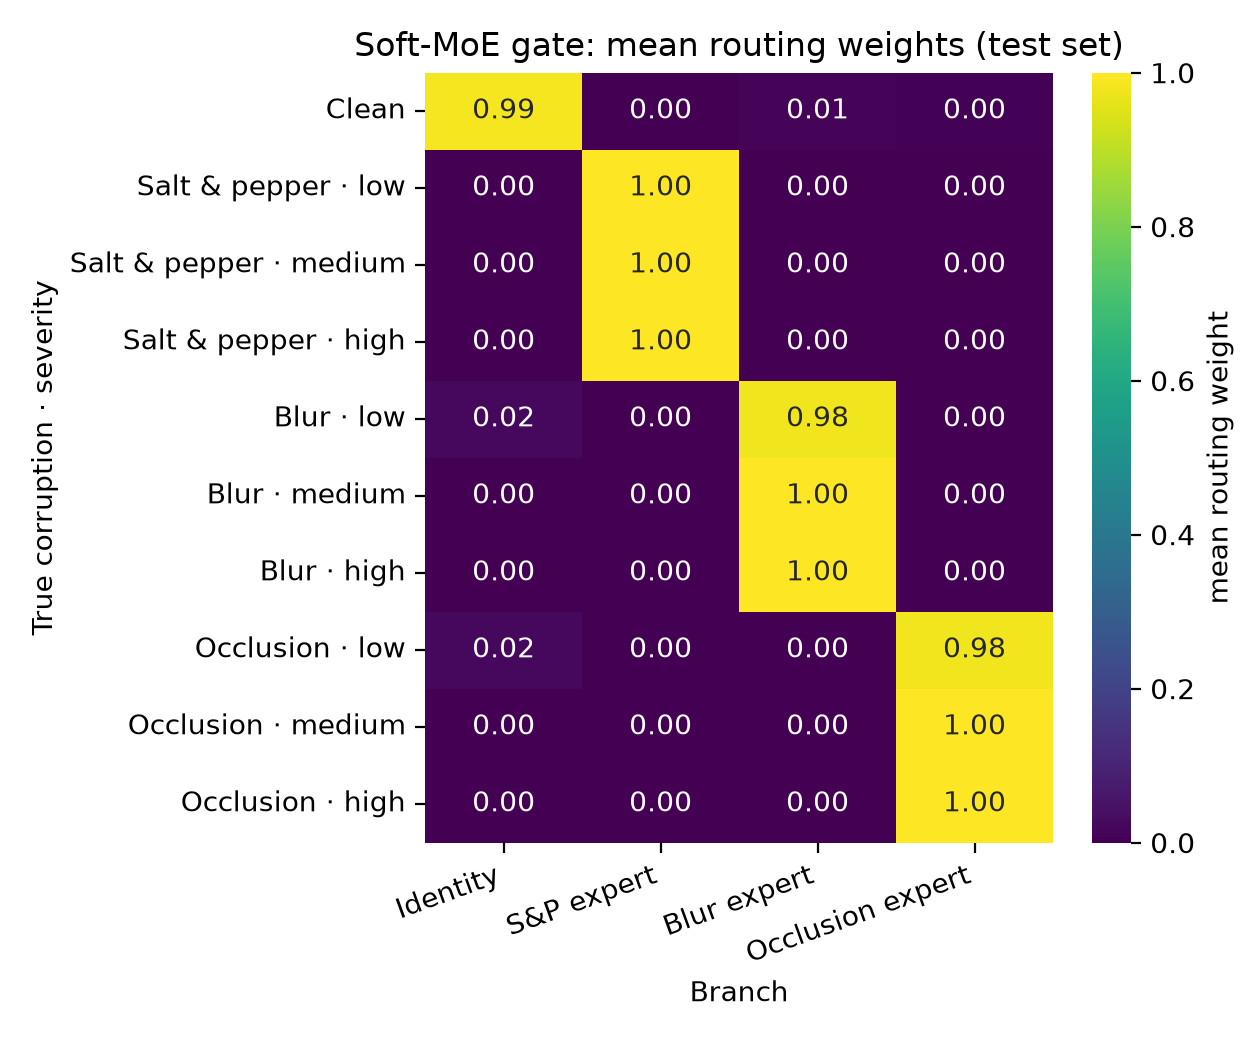
\includegraphics[width=0.9\columnwidth]{t3_heatmap.png}
\caption{Mean routing weight per true corruption and severity (test set).}\label{fig:heat}
\end{figure}

\begin{figure}[t]\centering
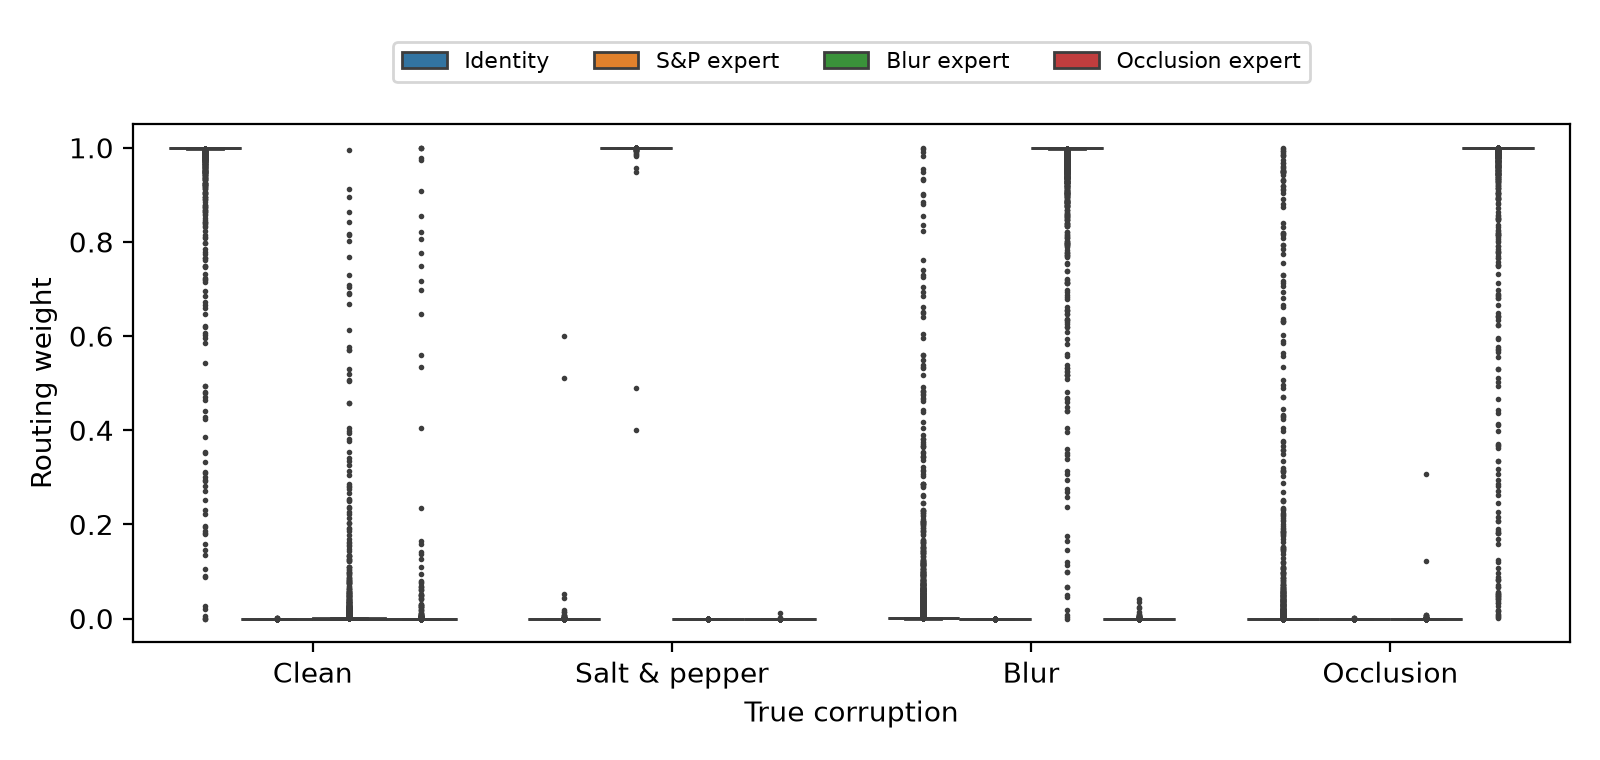
\includegraphics[width=\columnwidth]{t3_weights.png}
\caption{Distribution of routing weights per true corruption.}\label{fig:wdist}
\end{figure}

\begin{figure}[t]\centering
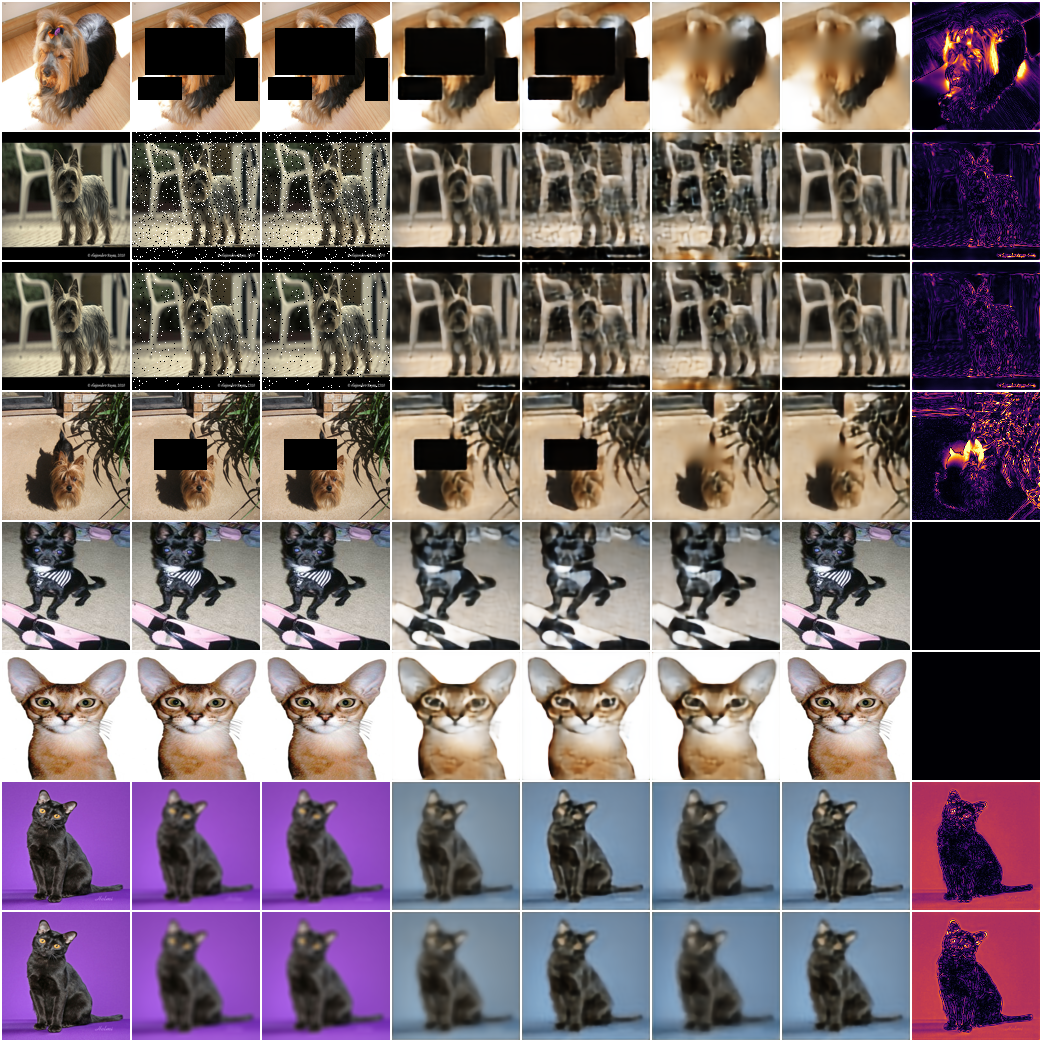
\includegraphics[width=\columnwidth]{t3_dominant.png}\\[1mm]
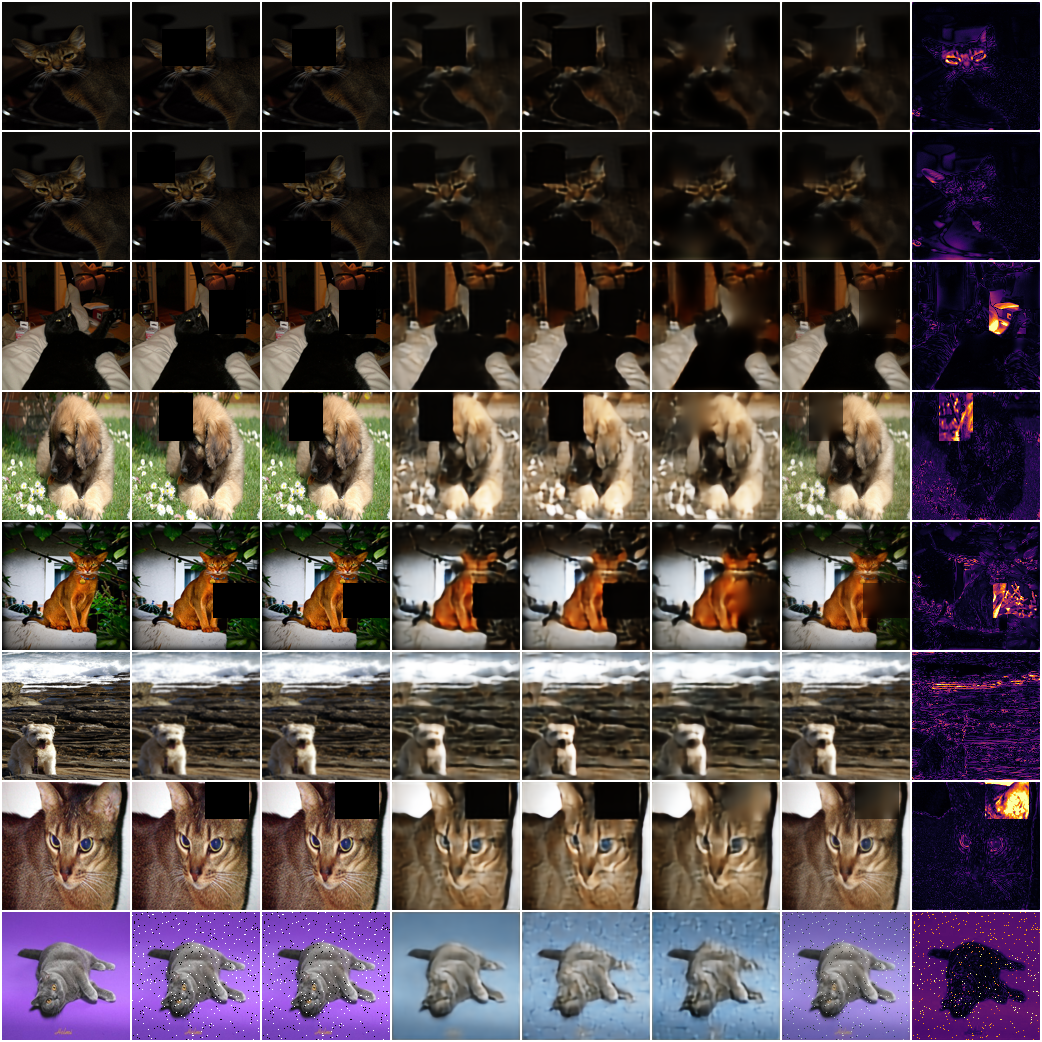
\includegraphics[width=\columnwidth]{t3_distributed.png}
\caption{Dominant-expert examples (top) and the most distributed examples (bottom). Columns: clean,
input, identity, S\&P, blur and occlusion expert outputs, MoE output, error. The distributed cases are
low-severity inputs split about 50/50 between the identity and the matching expert.}\label{fig:dist}
\end{figure}

%=====================================================================
\section{Task 4: Style-Conditioned Face-to-Sketch cGAN}\label{sec:t4}
%=====================================================================
\subsection{Data}
We use the official FS2K~\cite{fan2022fs2k} split (1,058 train / 1,046 test). Fifteen percent of the
training portion is held out with seed 42, stratified by style (899/159; per-style 303/298/298 and
54/52/53). Photos and sketches are resized to $128\times128$. The sketch path is derived from the photo
path exactly as in the official split script, which guarantees correct pairing. Augmentation upsamples
\emph{both} images to $142^2$, takes the \emph{same} random crop and applies the \emph{same} flip.
Independent transforms would destroy the pixel correspondence that the L1 term relies on.

\subsection{Architecture}
\textbf{Generator} $G(x,s)$: a 7-level U-Net~\cite{ronneberger2015unet} ($128\to1$) with full skip
connections, as in pix2pix. Skips are appropriate here, unlike in Task~1, because the output must stay
spatially aligned with the input. A learned embedding $e_s=\text{Emb}(s)\in\mathbb{R}^d$ enters the
network in two ways: it is concatenated to the $1\times1$ bottleneck, and it is mapped to per-channel
FiLM~\cite{perez2018film} scale and shift in every decoder block (zero-initialised, so training starts
from the unconditional model). Bottleneck concatenation lets the style affect global layout, and FiLM
lets it change stroke texture at every scale. We prefer this to input-only concatenation, which the
encoder can learn to ignore. Dropout in the first three decoder blocks provides stochasticity.
\textbf{Discriminator} $D(x,y,s)$: a $70\times70$ PatchGAN on $(x,y)$ concatenated with a projected,
spatially tiled style map, so a sketch counts as ``real'' only for its own style. It outputs a
$14\times14$ grid of patch logits. With the selected base width of 48 channels and a 16-dimensional
embedding, the generator has \textbf{23,678,403 parameters} and the discriminator \textbf{1,563,621}
(Fig.~\ref{fig:gan}).

\begin{figure}[t]\centering
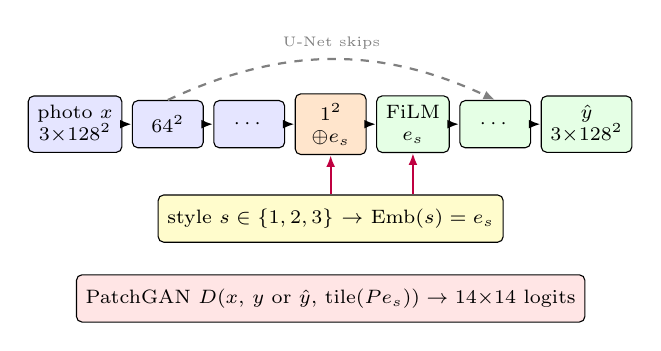
\begin{tikzpicture}[node distance=1.2mm]
\node[enc] (p) {photo $x$\\$3{\times}128^2$};
\node[enc, right=of p] (d1) {$64^2$};
\node[enc, right=of d1] (d2) {$\cdots$};
\node[lat, right=of d2] (b) {$1^2$\\$\oplus e_s$};
\node[dec, right=of b] (u1) {FiLM\\$e_s$};
\node[dec, right=of u1] (u2) {$\cdots$};
\node[dec, right=of u2] (y) {$\hat y$\\$3{\times}128^2$};
\foreach \a/\b in {p/d1,d1/d2,d2/b,b/u1,u1/u2,u2/y} \draw[arr] (\a) -- (\b);
\draw[arr, gray, dashed] (d1.north) to[bend left=25] node[above, font=\tiny]{U-Net skips} (u2.north);
\node[blk, fill=yellow!20, below=5mm of b] (s) {style $s\in\{1,2,3\}$ $\to$ Emb$(s)=e_s$};
\draw[arr, purple] (s) -- (b);
\draw[arr, purple] (s.north -| u1.south) -- (u1.south);
\node[blk, fill=red!10, below=4mm of s] (D) {PatchGAN $D(x,\,y\text{ or }\hat y,\,\text{tile}(Pe_s))\to 14{\times}14$ logits};
\end{tikzpicture}
\caption{Style-conditioned pix2pix. The style embedding enters the generator at the bottleneck
(concatenation) and in every decoder block (FiLM), and enters the discriminator as tiled input
channels.}
\label{fig:gan}
\end{figure}

\subsection{Objective and training}
$\mathcal{L}_D=\tfrac12[\text{BCE}(D(x,y,s),1)+\text{BCE}(D(x,G(x,s),s),0)]$ and
$\mathcal{L}_G=\text{BCE}(D(x,G(x,s),s),1)+\lambda_{L1}\lVert y-G(x,s)\rVert_1$, optimised with Adam
($\beta_1=0.5$), a constant learning rate for the first half of training and linear decay to zero over
the second half, and pix2pix initialisation. We log $D_{\text{real}}$, $D_{\text{fake}}$, $G_{\text{adv}}$,
$G_{L1}$ and validation L1/PSNR/SSIM separately. A fixed set of eight validation photographs is
rendered every five epochs in its own style and in all three styles.

\subsection{Optuna}
The search space covers generator and discriminator learning rates, batch size, base channels,
dropout, embedding dimension and $\lambda_{L1}\in[10,200]$ (log). Four 6-epoch trials
(compute-limited) were run, using the validation objective $\frac12\text{SSIM}+\frac12(1-\text{L1})$. The best
(0.666) used $\text{lr}_G=2{\cdot}10^{-4}$, a discriminator about 3$\times$ slower
($\text{lr}_D=6{\cdot}10^{-5}$), batch 4, 48 base channels, dropout 0.15, a 16-dimensional style embedding and
$\lambda_{L1}=44$. The two trials in which the discriminator learned faster than the generator scored
lowest (0.63), consistent with the usual advice not to let $D$ overpower $G$. The selected
configuration was retrained for 40 epochs (reduced from the planned 150 because of the deadline).
Fig.~\ref{fig:optgan} shows the study.

\begin{figure}[t]\centering
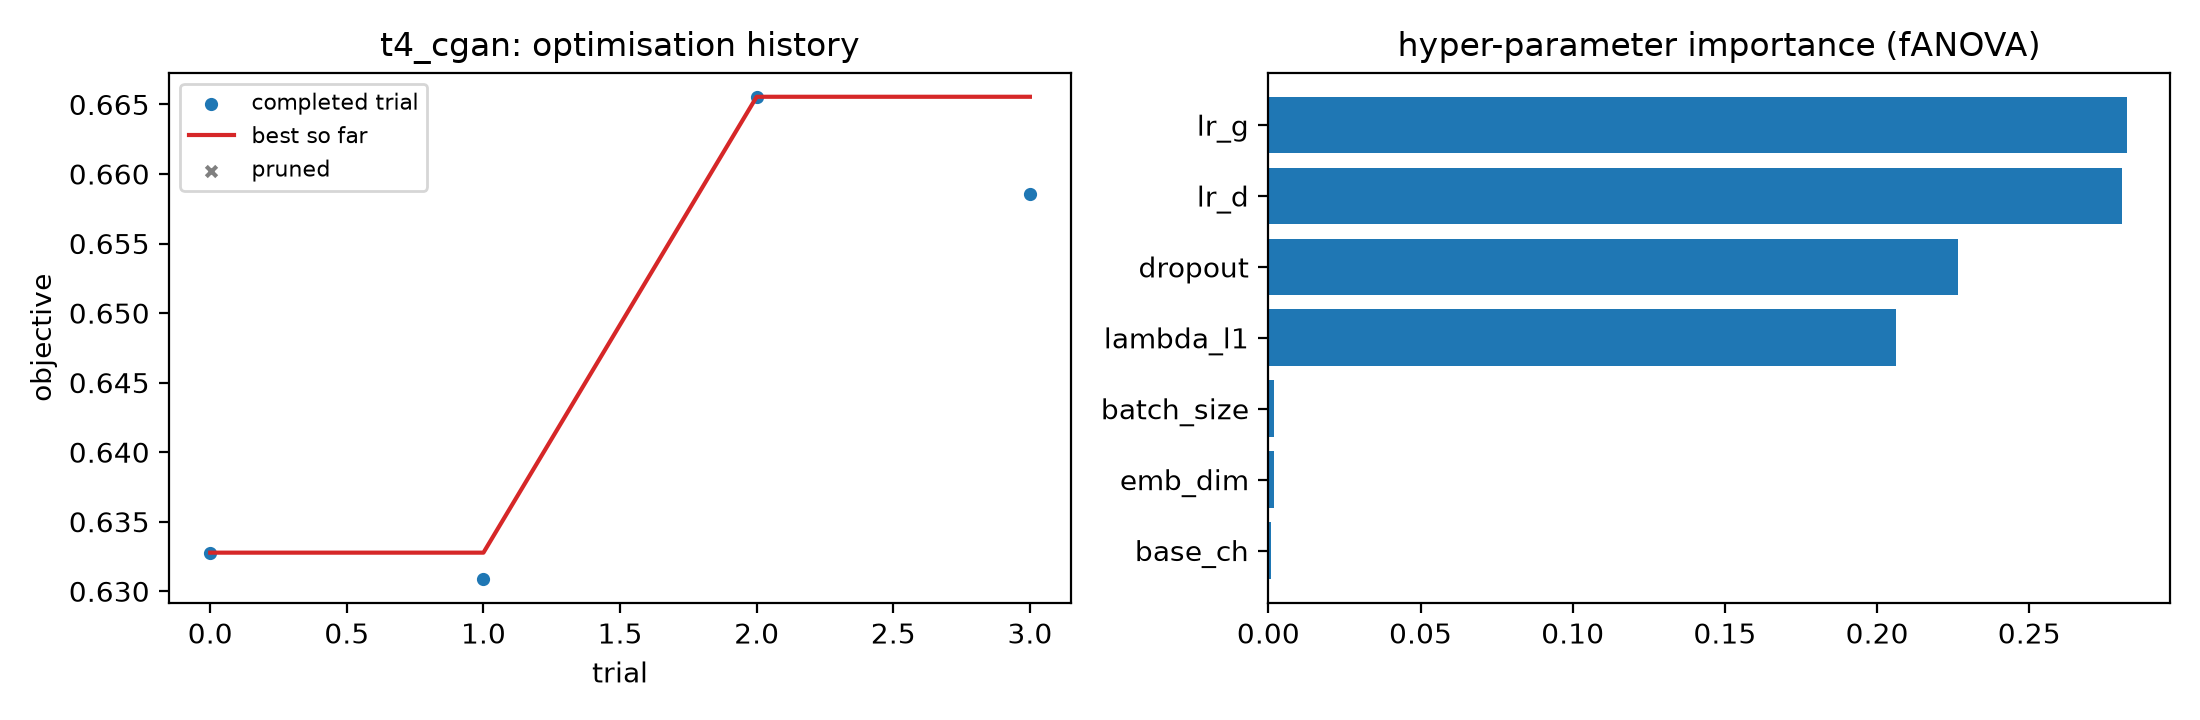
\includegraphics[width=\columnwidth]{optuna_t4_cgan.png}
\caption{Task 4 Optuna study (4 trials of 6 epochs).}\label{fig:optgan}
\end{figure}

\subsection{Results}
\textbf{Training dynamics} (Fig.~\ref{fig:t4curves}). Training was stable: $D_{\text{real}}$ and
$D_{\text{fake}}$ stayed balanced around 0.55--0.58 for all 40 epochs, with no discriminator
domination and no mode collapse. $G_{L1}$ fell from 0.30 to 0.19 and validation SSIM rose from 0.41
to 0.47. The fixed validation grid (Fig.~\ref{fig:t4grid}) shows the generator's progress: by epoch 40
it produces clean sketches that keep identity, hairstyle and accessories such as caps and earrings.

\textbf{Style conditioning.} The style sweep in Fig.~\ref{fig:t4grid} shows that the embedding controls
the output rather than being ignored: \emph{Style~1} gives light, thin outlines; \emph{Style~2} gives
dark, heavy hair and shading strokes; and \emph{Style~3} gives a grey, paper-like background with soft
shading. Each matches its artist's style in the training data.

\begin{table}[t]\centering\caption{Task 4 on the official FS2K test split.}\label{tab:t4}\footnotesize
\begin{tabular}{@{}lrrrrr@{}}\toprule
Style & L1 $\downarrow$ & PSNR $\uparrow$ & SSIM $\uparrow$ & FID $\downarrow$ & $n$\\\midrule
Style 1 & 0.084 & 16.98 & 0.493 & 91.9 & 619\\
Style 2 & 0.155 & 12.35 & 0.370 & 76.9 & 381\\
Style 3 & 0.070 & 18.19 & 0.592 & -- & 46\\\midrule
Overall & 0.109 & 15.35 & 0.453 & 78.2 & 1,046\\\bottomrule
\end{tabular}\end{table}

\textbf{Metrics} (Table~\ref{tab:t4}). Pixel metrics and FID disagree in an informative way. Style~2,
with heavy strokes, has the \emph{worst} L1/SSIM but the \emph{best} FID: dense dark strokes are almost
impossible to reproduce at the same pixel positions, yet their overall statistics are easy to imitate.
Style~3's sketches are mostly flat grey and score best on pixel metrics. FID is not reported for
Style~3 because only 46 test images exist (the official test split is heavily unbalanced, 619/381/46),
and a 2048-dimensional covariance estimate from 46 samples would be meaningless.

\textbf{Failure cases} (Fig.~\ref{fig:t4fail}). The lowest-SSIM test images are all subjects with long,
voluminous hair. The artist draws hair as dense individual strokes, and the generator produces
plausible strands that are not at the same pixel positions. The sketches look reasonable, but SSIM
drops to 0.16--0.18. This is the main weakness of paired pixel losses for line art. A second failure
type is out-of-distribution faces: heavy face paint (the last row of Fig.~\ref{fig:t4grid}) breaks
the facial structure and produces fragmented strokes. Very light blonde hair against a light background
is sometimes drawn too faintly.

\begin{figure}[t]\centering
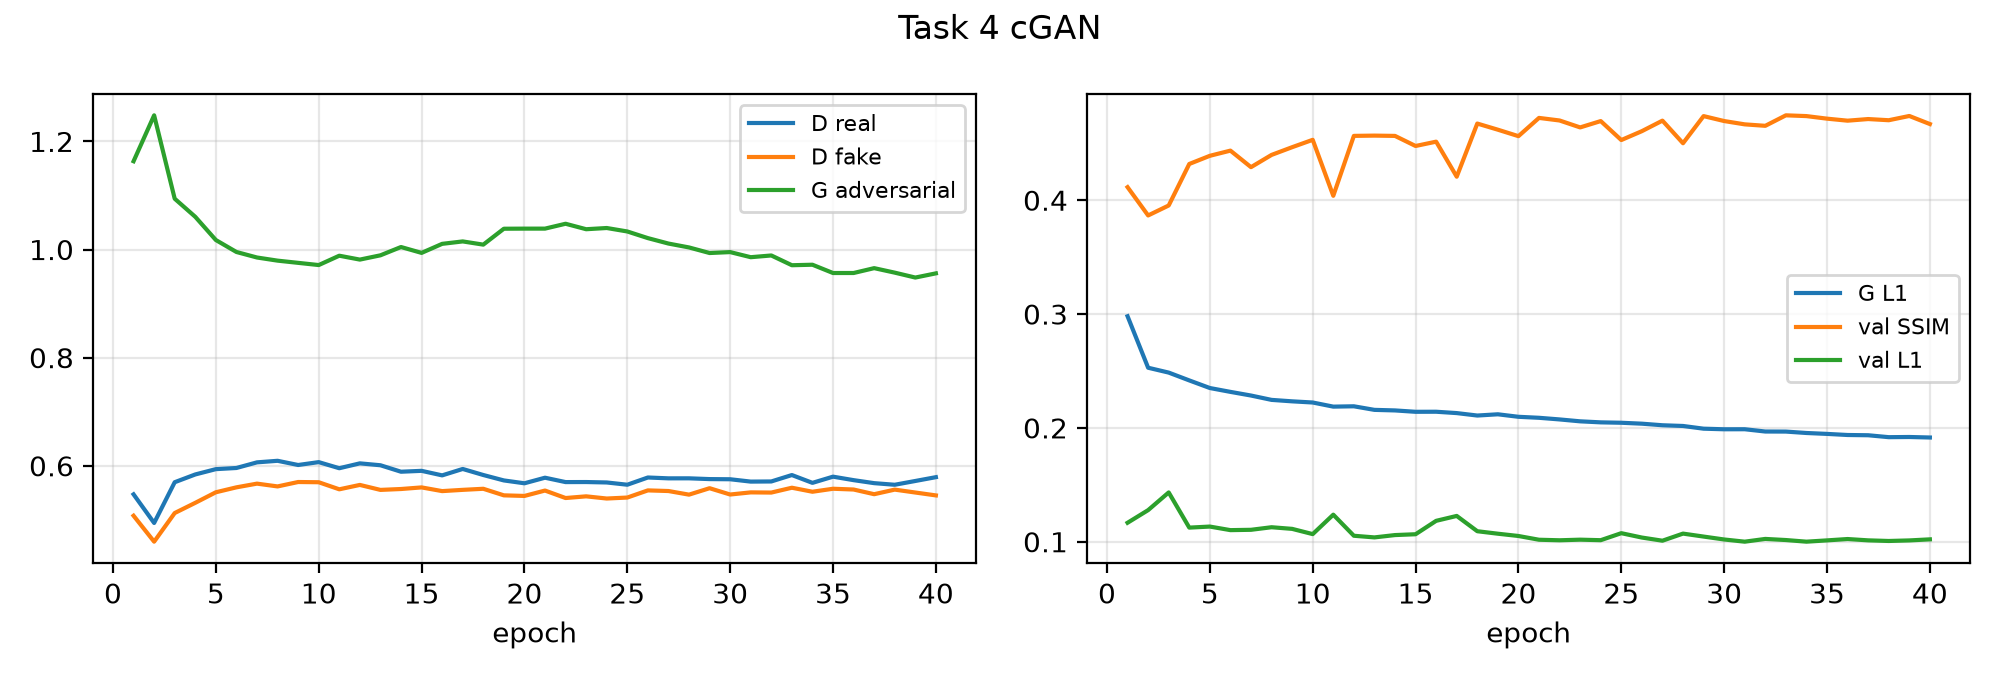
\includegraphics[width=\columnwidth]{t4_curves.png}
\caption{Task 4 training: discriminator real/fake loss, generator adversarial and L1 loss, validation
SSIM and L1 (all logged separately in MLflow).}\label{fig:t4curves}
\end{figure}

\begin{figure}[t]\centering
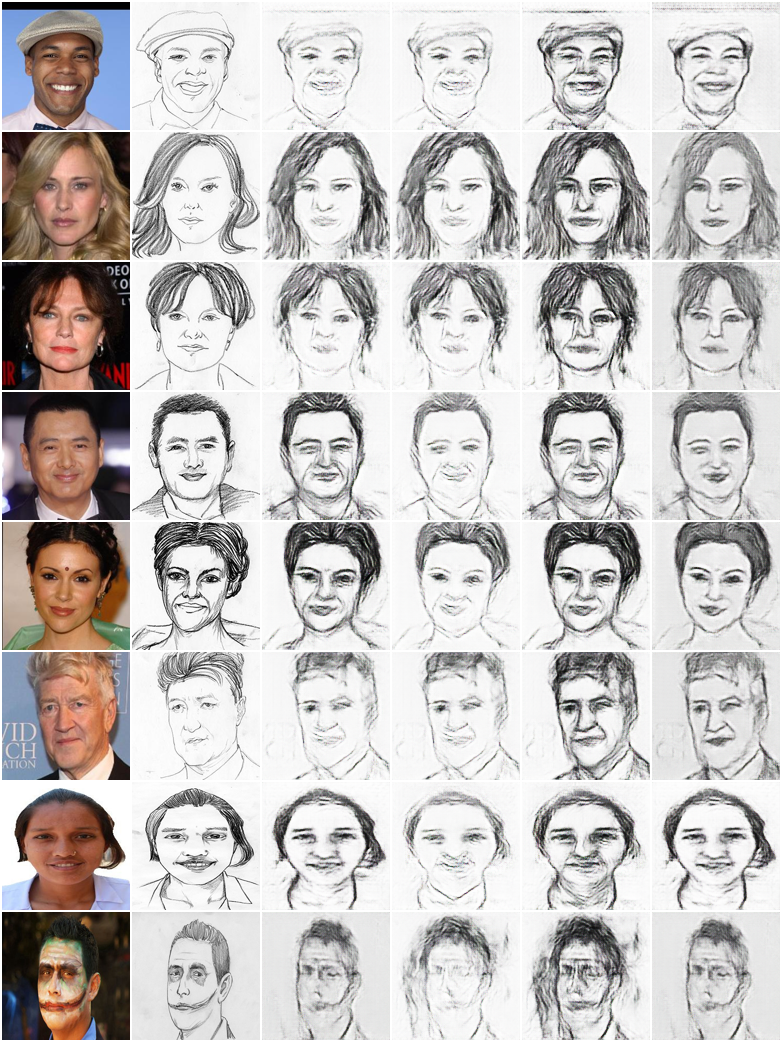
\includegraphics[width=0.95\columnwidth]{t4_fixed_val.png}
\caption{Fixed validation photographs at epoch 40. Columns: photo, ground truth, generated in its own
style, then Style~1, Style~2 and Style~3 for the same photo.}\label{fig:t4grid}
\end{figure}

\begin{figure}[t]\centering
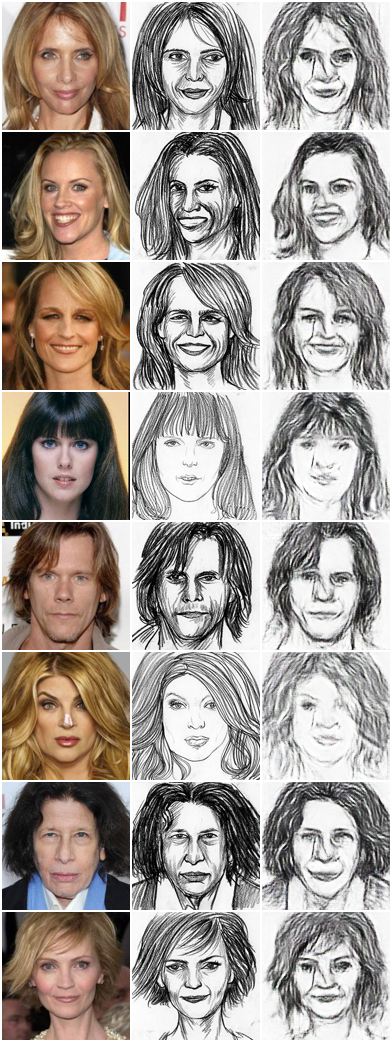
\includegraphics[width=0.45\columnwidth]{t4_failures.png}
\caption{Lowest-SSIM test cases (photo, ground truth, generated): plausible but misaligned hair
strokes.}\label{fig:t4fail}
\end{figure}

\begin{figure}[t]\centering
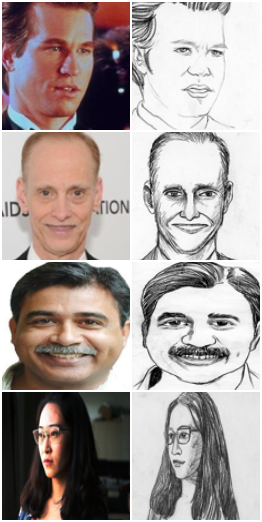
\includegraphics[width=0.3\columnwidth]{fs2k_pairs.png}
\caption{FS2K training pairs after identical paired augmentation (photo, target sketch).}
\label{fig:fs2k}
\end{figure}

%=====================================================================
\section{Application and Deployment}\label{sec:app}
%=====================================================================
\textbf{Design.} The interface uses a top
navigation bar with the four named workspaces, a 340px control column and a results area. The design
tokens (indigo accent, 16px cards, Inter typeface) are defined once in Tailwind's \texttt{@theme}.

\textbf{Backend.} FastAPI loads the seven ONNX models at start-up with ONNX Runtime and warms them up.
It exposes \texttt{/api/health}, \texttt{/api/info}, \texttt{/api/samples}, \texttt{/api/corrupt},
\texttt{/api/restore/\{universal,hard,soft\}} and \texttt{/api/sketch}. Uploads are validated by MIME
type, size ($\le$10\,MB), decodability and minimum size, then EXIF-transposed and resized. The
corruption code used for runtime corruption in the app is \emph{the same module} used for training
(NumPy-only, so the backend image needs no PyTorch). Responses carry the images, the corruption
parameters, classifier probabilities or routing weights, PSNR when a clean reference is known, and
timing broken down by stage.

\textbf{Frontend.} React~19, TypeScript and Tailwind~4 (Vite). Each workspace supports sample
selection, drag-and-drop upload (and webcam capture for faces), corruption type, severity or custom
parameters with a seed, oracle versus predicted routing, probability and weight bars, a stacked
contribution bar, error maps and result download.

\textbf{Containers.} \texttt{docker compose up --build} starts the backend (Python 3.12 slim, uv-locked
dependencies, health check) and the frontend (multi-stage Node build served by nginx, which proxies
\texttt{/api}). Models are mounted read-only from \texttt{./models}. The backend reports every expected
model file in \texttt{/api/health}; a workspace whose model is missing fails gracefully with HTTP 503
and is listed as ``missing'' on the Overview page. Eleven
API tests (validation, path-traversal protection, oracle versus predicted routing, weights summing to one,
all three sketch styles) run against ONNX models with the production signatures.

\textbf{ONNX parity.} Each exported model was run on real validation images in PyTorch and ONNX
Runtime (CPU). Maximum absolute differences: universal DAE $3.6{\times}10^{-6}$; classifier logits
$3.3{\times}10^{-6}$; specialists $2.4{\times}10^{-6}$ (S\&P), $1.5{\times}10^{-6}$ (blur) and
$1.2{\times}10^{-5}$ (occlusion); soft MoE $3.7{\times}10^{-6}$ (restored), $5{\times}10^{-10}$
(weights); sketch generator $2.0{\times}10^{-6}$. All are within float32 round-off.

\textbf{Screenshots.} Fig.~\ref{fig:app} shows the running application (Docker Compose, Chromium,
previously unseen test images). Each workspace shows the input, the output, the routing information
and the timing.

\begin{figure*}[t]\centering

\includegraphics[width=0.49\textwidth]{app_universal.png}\hfill
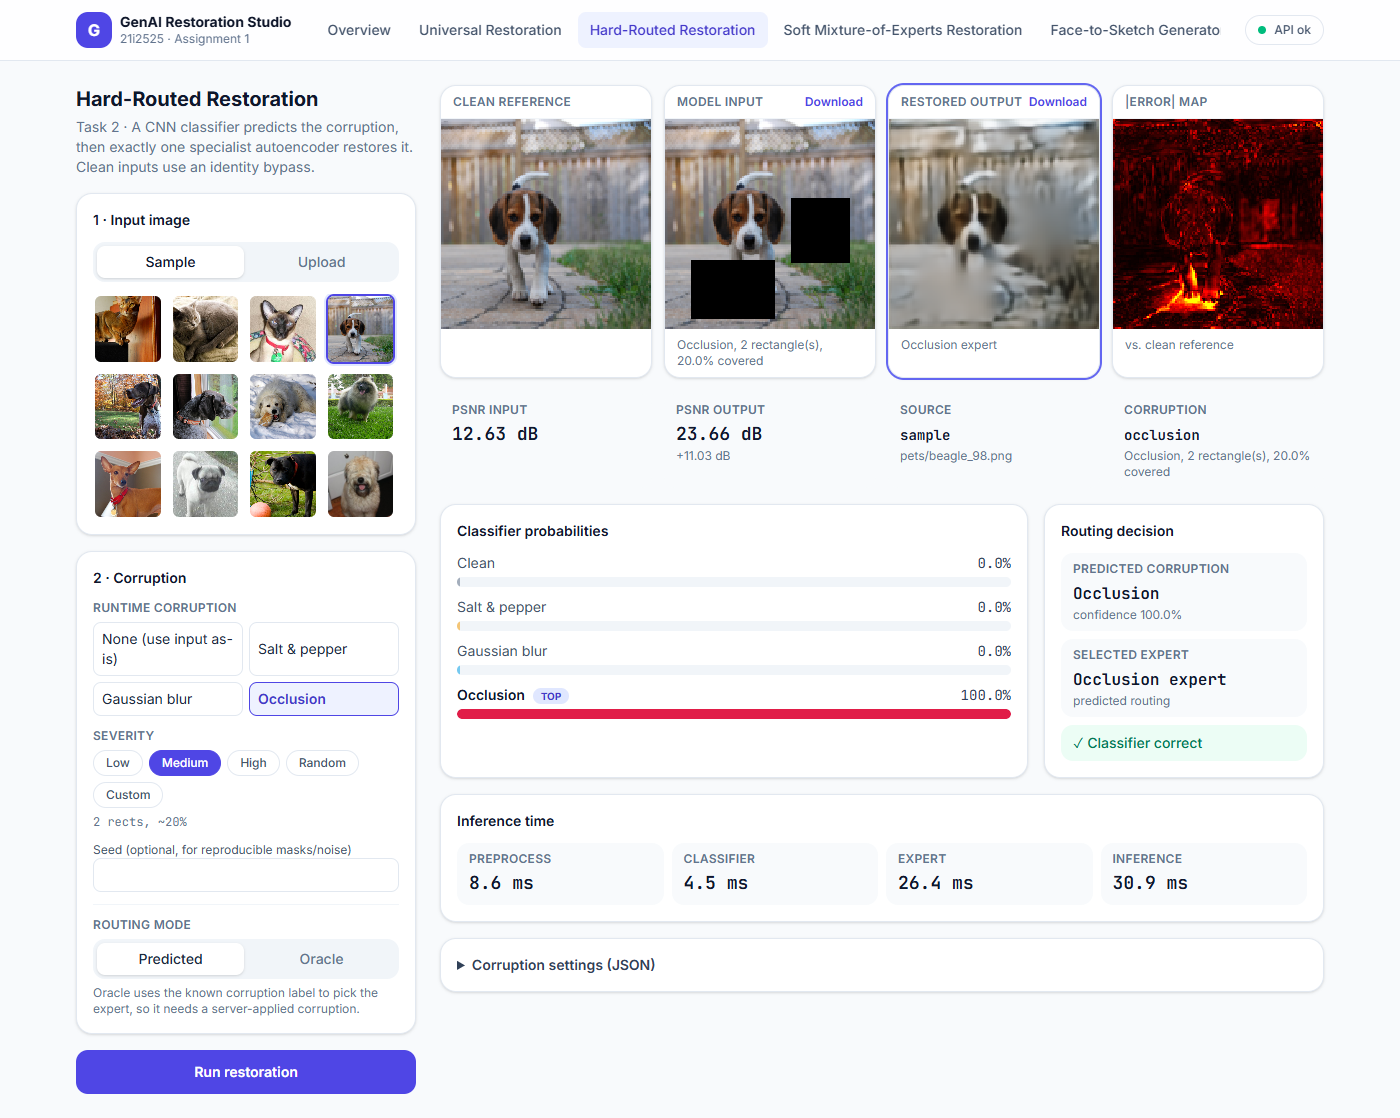
\includegraphics[width=0.49\textwidth]{app_hard.png}\\[2mm]

\includegraphics[width=0.49\textwidth]{app_soft.png}\hfill
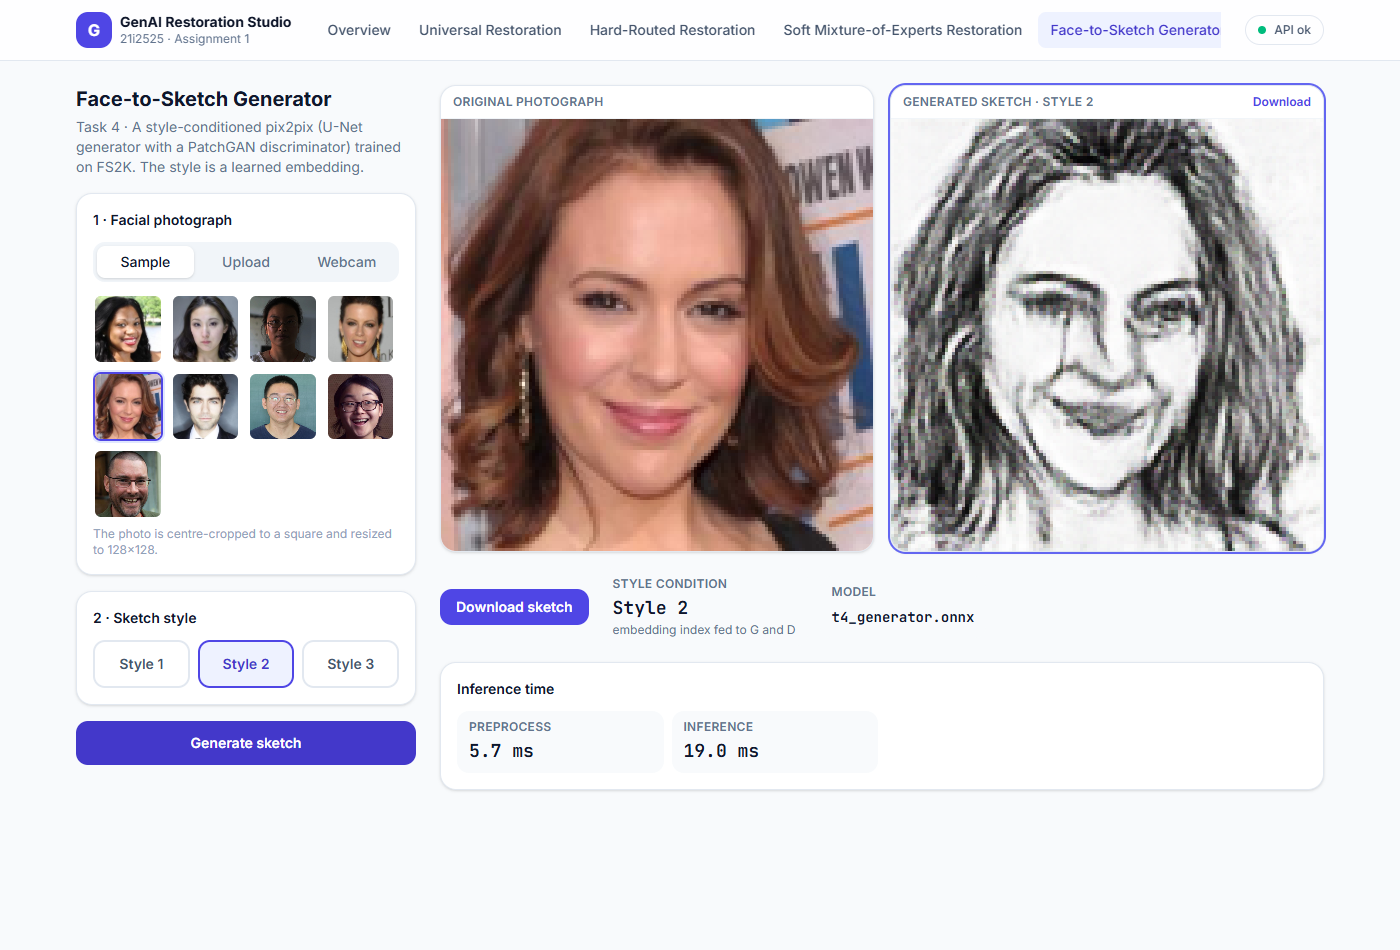
\includegraphics[width=0.49\textwidth]{app_sketch.png}
\caption{The deployed application. Top left: Universal Restoration (input, output, error map, PSNR,
timing). Top right: Hard-Routed Restoration (classifier probabilities, selected expert). Bottom left:
Soft Mixture-of-Experts (routing weights and contribution bar). Bottom right: Face-to-Sketch
Generator (style selection, side-by-side output, download).}\label{fig:app}
\end{figure*}


%=====================================================================
\section{Limitations}
%=====================================================================
(1)~\emph{Short schedules}: the specialists (20 epochs), the MoE joint stage and the GAN were trained
with deadline-reduced budgets, and the Task~3 and~4 Optuna studies used only four trials.
(2)~\emph{Budgets}: Optuna trials were short (6--15 epochs) on a 4\,GB laptop GPU, and we observed
short-horizon bias directly. (3)~\emph{Bottleneck ceiling}: about 26.5\,dB at $128\times128$; the
planned skip ablation was not run. (4)~\emph{Occlusion is inpainting}, and L1+SSIM produces blurry fills.
A perceptual or adversarial term would help. (5)~\emph{Engineering}: on Windows, every DataLoader
worker re-imports CUDA (about 2\,GB commit each). Leaked persistent workers stalled training until we
added explicit worker shutdown. Per-sample GPU$\to$CPU transfers made evaluation take over 2\,h until we
batched them (90\,s after the fix).

%=====================================================================
\section{Conclusion and Future Work}
%=====================================================================
\textbf{Task 1.} A single autoencoder with a genuine 8,192-value bottleneck removes impulse noise very
effectively (+13\,dB at $p=0.15$) and raises corrupted-input PSNR from 19.3 to 24.6\,dB. Its weaknesses
are a fidelity ceiling of about 26.5\,dB, which degrades clean and lightly blurred images, and blurry
inpainting of occlusions. \emph{Future work}: run the limited-skip ablation, and add a perceptual or
adversarial term for occlusion.

\textbf{Task 2.} The corruption classifier is almost perfect (99.82\% accuracy, macro-F1 0.997), so
predicted routing equals oracle routing to within 0.02\,dB. The identity bypass removes the clean-image
penalty. Hard routing is only as good as its experts, and its rare errors (black backgrounds mistaken
for occlusion) are its most damaging failures. The second, longer Optuna study showed and corrected
short-horizon bias. \emph{Future work}: train the specialists as long as the universal model, and add an
``uncertain $\Rightarrow$ identity'' fallback.

\textbf{Task 3.} Initialised from Task~2, the jointly trained soft MoE learns near-hard routing
(99.0\% of images with one weight $\ge0.9$), has no inactive or dominating experts, and hedges only on
low-severity and mixed inputs, where it beats hard routing. \emph{Future work}: train the experts on
corruption mixtures, use a longer joint stage with a smaller $\lambda_c$, and run a larger Optuna budget.

\textbf{Task 4.} The style-conditioned pix2pix trains stably, keeps identity and produces three
visibly distinct sketch styles from one generator (overall FID 78.2). Pixel metrics penalise plausible
but misaligned hair strokes. \emph{Future work}: the full 150-epoch schedule, perceptual or LPIPS
losses, and style-balanced sampling, given only 46 Style-3 test images.

All code, configurations, Optuna studies, MLflow records and ONNX models are in the repository.

\bibliographystyle{IEEEtran}
\bibliography{references}

\appendices
\section{Use of AI Assistants}
\textbf{Tool.} Claude Code (Anthropic, Claude Opus model), an AI coding assistant, used inside VS Code.

\textbf{Used for.} Reading the brief into a requirements checklist; drafting the data pipeline,
models, training and Optuna scripts, evaluation, ONNX export, FastAPI backend, React UI, Dockerfiles,
README and this report; debugging; looking up the FS2K split layout and the
SciPy/Tailwind API changes.

\textbf{Verification and corrections.} (i)~Unit tests check every corruption against the specification
(S\&P fraction and 50/50 colours, occlusion coverage $\pm$1\%, blur equal to \texttt{torchvision} to
$<10^{-5}$) and the determinism of the manifests. Eleven API tests cover the backend. (ii)~Every eval
and export script was dry-run on untrained models before the real runs; this caught four bugs:
infinite PSNR on identity-restored clean images inflating averages, an empty-grid crash, a removed
SciPy argument, and a network-dependent FID failure. (iii)~ONNX parity is checked numerically for
every model. (iv)~Figures of corruptions, FS2K pairs, failures and misroutes were inspected visually.
(v)~Experiment results led to design corrections: the $8\times8$ latent plateau (latent resolution
added to the search), short-horizon bias (second specialist study), Windows worker leaks and
per-sample GPU syncs (fixed and documented above). The author reviewed the generated code and is
responsible for it.

\end{document}
